\chapter{Solving Linear Equations} \label{lineq}

\normalsize

The primary motivation for the study of vectors and matrices is based
on the study of solving systems of linear equations.  The algorithms
that enable us to find solutions are themselves based on certain kinds
of matrix manipulations.  In these algorithms, matrices serve as a
shorthand for calculation, rather than as a basis for a theory.  We will
see later that these matrix manipulations do lead to a rich theory of how
to solve systems of linear equations.  But our first step is just to see
how these equations are actually solved.

We begin with a discussion in Section~\ref{S:2.1} of how to write systems
of linear equations in terms of matrices.  We also show by example how
complicated writing down the answer to such systems can be.  In
Section~\ref{S:2.2}, we recall that solution sets to systems of linear
equations in two and three variables are lines and planes.

The best known and probably the most efficient method for solving
systems of linear equations (especially with a moderate to large number
of unknowns) is Gaussian elimination.  The idea behind this method,
which is introduced in Section~\ref{S:Gauss}, is to manipulate matrices
by elementary row operations to reduced echelon form.  It is then possible
just to look at the reduced echelon form matrix and to read off the
solutions to the linear system, if any.  The process of reading off the
solutions is formalized in Section~\ref{S:2.4}; see Theorem~\ref{number}.
Our discussion of solving linear equations is presented with equations
whose coefficients are real numbers --- though most of our examples have
just integer coefficients.  The methods work just as well with complex
numbers, and this generalization is discussed in Section~\ref{S:specialcoeff}.

Throughout this chapter, we alternately discuss the theory and show how
calculations that are tedious when done by hand can easily be performed
by computer using \Matlabp.  The chapter ends with a proof of the
uniqueness of row echelon form (a topic of theoretical importance) in
Section~\ref{S:uniquerowechelon}.  This section is included mainly for
completeness and need not be covered on a first reading.


\section{Systems of Linear Equations and Matrices}
\label{S:2.1}

It is a simple exercise to solve the system of two equations
\begin{equation} \label{small}
\arraycolsep 2pt
\begin{array}{rcrcr}
 x & + & y & = & 7 \\
-x & + & 3y & = & 1
\end{array}
\end{equation}
to find that $x=5$ and $y=2$.  One way to solve
system \Ref{small} is to add the two equations, obtaining
\[
4y=8;
\]
hence $y=2$.  Substituting $y=2$ into the $1^{st}$ equation in
\Ref{small} yields $x=5$.

This system of equations can be solved in a more algorithmic
fashion by solving the $1^{st}$ equation in \Ref{small} for $x$
as
\[
x = 7 - y,
\]
and substituting this answer into the $2^{nd}$ equation in
\Ref{small}, to obtain
\[
-(7-y) +3y = 1.
\]
This equation simplifies to:
\[
4y = 8.
\]
Now proceed as before.

\subsection*{Solving Larger Systems by Substitution}

In contrast to solving the simple system of two equations,
it is less clear how to solve a complicated system of five
equations such as:
\begin{equation}    \label{big}
\arraycolsep 2pt
\begin{array}{rcrcrcrcrcrl}
 5x_1 & - & 4x_2 & + & 3x_3 & - & 6x_4 & + & 2x_5 & = &   4  & \\
 2x_1 & + &  x_2 & - &  x_3 & - &  x_4 & + &  x_5 & = &   6  & \\
  x_1 & + & 2x_2 & + &  x_3 & + &  x_4 & + & 3x_5 & = &  19  & \\
-2x_1 & - &  x_2 & - &  x_3 & + &  x_4 & - &  x_5 & = & -12  & \\
  x_1 & - & 6x_2 & + &  x_3 & + &  x_4 & + & 4x_5 & = &   4  & \!
.
\end{array}
\end{equation}
The algorithmic method used to solve \Ref{small} can be expanded
to produce a method, called {\em substitution\/},
\index{substitution} for solving larger systems. We describe the
substitution method as it applies to \Ref{big}.  Solve the
$1^{st}$ equation in \Ref{big} for $x_1$, obtaining
\begin{equation} \label{x1}
x_1 = \frac{4}{5}  + \frac{4}{5}x_2 - \frac{3}{5}x_3
   + \frac{6}{5}x_4 - \frac{2}{5}x_5.
\end{equation}
Then substitute the right hand side of \Ref{x1} for $x_1$ in the
remaining four equations in \Ref{big} to obtain a new system of
four equations in the four variables $x_2$,$x_3$,$x_4$,$x_5$.
This procedure eliminates the variable $x_1$.  Now proceed
inductively --- solve the $1^{st}$ equation in the new system
for $x_2$ and substitute this expression into the remaining
three equations to obtain a system of three equations in three
unknowns.  This step eliminates the variable $x_2$.  Continue by
substitution to eliminate the variables $x_3$ and $x_4$, and
arrive at a simple equation in $x_5$ --- which can be solved.
Once $x_5$ is known, then $x_4$, $x_3$, $x_2$, and $x_1$ can be
found in turn.

\subsection*{Two Questions}

\begin{itemize}
\item Is it realistic to expect to complete the substitution
procedure without making a mistake in arithmetic?
\item Will this procedure work --- or will some unforeseen
difficulty arise?
\end{itemize}

Almost surely, attempts to solve \Ref{big} by hand,
using the substitution procedure, will lead to arithmetic
errors.  However, computers and software have developed to the
point where solving a system such as \Ref{big} is routine.  In
this text, we use the software package \Matlab to illustrate
just how easy it has become to solve equations such as \Ref{big}.

The answer to the second question requires knowledge of the
{\em theory\/} of linear algebra.  In fact, no difficulties will
develop when trying to solve the particular system \Ref{big}
using the substitution algorithm.  We discuss why later.

\subsection*{Solving Equations by \Matlab}

We begin by discussing the information that is needed by \Matlab
to solve \Ref{big}.  The computer needs to know that there are
five equations in five unknowns --- but it does not need to keep
track of the unknowns $(x_1,x_2,x_3,x_4,x_5)$ by name.  Indeed,
the computer just needs to know the {\em matrix of
coefficients\/} \index{matrix!coefficient} in \Ref{big}
\begin{equation*}  \label{bigmatrix}
\left(
\begin{array}{rrrrr}
 5 & -4 &  3 & -6 &  2 \\
 2 &  1 & -1 & -1 &  1 \\
 1 &  2 &  1 &  1 &  3 \\
-2 & -1 & -1 &  1 & -1 \\
 1 & -6 &  1 &  1 &  4
\end{array}
\right)
\end{equation*}
and the {\em vector\/} on the right hand side of \Ref{big}
\begin{equation*} \label{bigRHS}
\left(
\begin{array}{r}
  4 \\
  6 \\
 19 \\
-12 \\
  4
\end{array}
\right).
\end{equation*}

We now describe how we enter this information into \Matlabp.  To
reduce the drudgery and to allow us to focus on ideas, the entries
in equations having a $*$ after their label
(such as \Ref{bigmatrix}*) have been entered in the {\tt laode}
toolbox. This information can be accessed as follows.  After
starting your \Matlab session, type
\begin{verbatim}
e2_1_4
\end{verbatim}
followed by a carriage return.  This instruction tells \Matlab to
load equation \Ref{bigmatrix} of Chapter~\ref{lineq}.  The matrix of
coefficients is now available in \Matlabp; note that this matrix is
stored in the $5\times 5$ array {\tt A}.  What should appear is:
\begin{verbatim}
A =
     5    -4     3    -6     2
     2     1    -1    -1     1
     1     2     1     1     3
    -2    -1    -1     1    -1
     1    -6     1     1     4
\end{verbatim}
Indeed, comparing this result with \Ref{bigmatrix}, we see that
{\tt A} contains precisely the same information.

Since the label \Ref{bigRHS} is followed by a `$*$', we can enter
the vector in \Ref{bigRHS} into \Matlab by typing
\begin{verbatim}
e2_1_5
\end{verbatim}
Note that the right hand side of \Ref{big} is stored in the vector {\tt b}.
\Matlab should have responded with
\begin{verbatim}
b =
     4
     6
    19
   -12
     4
\end{verbatim}
Now \Matlab has all the information it needs to solve the system
of equations given in \Ref{big}.  To have \Matlab solve this
system, type
\begin{verbatim}
x = A\b
\end{verbatim}
\index{\computer!$\backslash$}to obtain
\begin{verbatim}
x =
    5.0000
    2.0000
    3.0000
    4.0000
    1.0000
\end{verbatim}
This answer is interpreted as follows: the five values of the
unknowns $x_1$,$x_2$,$x_3$,$x_4$,$x_5$ are stored in the vector
$x$; that is,
\begin{equation} \label{answer1}
 x_1 = 5,\quad x_2 = 2,\quad x_3 = 3,\quad x_4 = 4,\quad x_5 = 1.
\end{equation}
The reader may verify that \Ref{answer1} is indeed a solution of
\Ref{big} by substituting the values in \Ref{answer1} into the
equations in \Ref{big}.

\subsection*{Changing Entries in \Matlab}

\Matlab also permits access to single components of $x$.  For
instance, type
\begin{verbatim}
x(5)
\end{verbatim}
and the $5^{th}$ entry of $x$ is displayed,
\begin{verbatim}
ans =
    1.0000
\end{verbatim}
We see that the component {\tt x(i)} of {\tt x} corresponds to
the component $x_i$ of the vector $x$ where $i=1,2,3,4,5$.
Similarly, we can access the entries of the coefficient matrix
\index{matrix!coefficient} {\tt A}.
For instance, by typing
\begin{verbatim}
A(3,4)
\end{verbatim}
\Matlab responds with
\begin{verbatim}
ans =
    1
\end{verbatim}

It is also possible to change an individual entry in either a vector
or a matrix.  For example, if we enter
\begin{verbatim}
A(3,4) = -2
\end{verbatim}  \index{\computer!A(3,4)}
we obtain a new matrix {\tt A} which when displayed is:
\begin{verbatim}
A =
     5    -4     3    -6     2
     2     1    -1    -1     1
     1     2     1    -2     3
    -2    -1    -1     1    -1
     1    -6     1     1     4
\end{verbatim}
Thus the command {\tt A(3,4) = -2} changes the entry in the
$3^{rd}$ row, $4^{th}$ column of {\tt A} from $1$ to $-2$.
In other words, we have now entered into \Matlab the
information that is needed to solve the system of equations
\[
\arraycolsep 2pt
\begin{array}{rcrcrcrcrcrl}
 5x_1 & - & 4x_2 & + & 3x_3 & - &  6x_4 & + & 2x_5 & = &   4  & \\
 2x_1 & + &  x_2 & - &  x_3 & - &   x_4 & + &  x_5 & = &   6  & \\
  x_1 & + & 2x_2 & + &  x_3 & - &  2x_4 & + & 3x_5 & = &  19  & \\
-2x_1 & - &  x_2 & - &  x_3 & + &   x_4 & - &  x_5 & = & -12  & \\
x_1 & - & 6x_2 & + & x_3 & + & x_4 & + & 4x_5 & = & 4 & \! .
\end{array}
\]
As expected, this change in the coefficient matrix results in a
change in the solution of system \Ref{big}, as well.  Typing
\begin{verbatim}
x = A\b
\end{verbatim}
now leads to the solution
\begin{verbatim}
x =
    1.9455
    3.0036
    3.0000
    1.7309
    3.8364
\end{verbatim}
that is displayed to an accuracy of four decimal places.

In the next step, change {\tt A} as follows:
\begin{verbatim}
A(2,3) = 1
\end{verbatim}
The new system of equations is:
\begin{equation}  \label{incon}
\arraycolsep 2pt
\begin{array}{rcrcrcrcrcrl}
 5x_1 & - & 4x_2 & + & 3x_3 & - &  6x_4 & + & 2x_5 & = &   4  & \\
 2x_1 & + &  x_2 & + &  x_3 & - &   x_4 & + &  x_5 & = &   6  & \\
  x_1 & + & 2x_2 & + &  x_3 & - &  2x_4 & + & 3x_5 & = &  19  & \\
-2x_1 & - &  x_2 & - &  x_3 & + &   x_4 & - &  x_5 & = & -12  & \\
  x_1 & - & 6x_2 & + &  x_3 & + &   x_4 & + & 4x_5 & = &   4  & \!
.
\end{array}
\end{equation}
The command
\begin{verbatim}
x = A\b
\end{verbatim}  \index{\computer!$\backslash$}
now leads to the message
\begin{verbatim}
Warning: Matrix is singular to working precision.

x =
   Inf
   Inf
   Inf
   Inf
   Inf
\end{verbatim}  \index{\computer!inf}
Obviously, something is {\em wrong\/}; \Matlab cannot find a
solution to this system of equations!  Assuming that \Matlab is
working correctly, we have shed light on one of our previous
questions: the method of substitution described by \Ref{x1} need
{\em not\/} always lead to a solution, even though the method
does work for system \Ref{big}.  Why?  As we will see, this is
one of the questions that is answered by the theory of linear
algebra.  In the case of \Ref{incon}, it is fairly easy to see
what the difficulty is: the second and fourth equations
have the form $y=6$ and $-y=-12$, respectively.

\vspace{0.1in}

\noindent {\bf Warning:}  The \Matlab command
\begin{verbatim}
x = A\b
\end{verbatim}
may give an error message similar to the previous one.  When
this happens, one must approach the answer with caution.

\EXER


\TEXER

\noindent In Exercises~\ref{c2.1.8a} -- \ref{c2.1.8c} find solutions
to the given system of linear equations.
\begin{exercise} \label{c2.1.8a}
\[
\begin{array}{rcrcr}
 2x & - & y & = & 0 \\
 3x &   &   & = & 6 \end{array}
\]
\end{exercise}
\begin{exercise} \label{c2.1.8b}
\[
\begin{array}{rcrcrcr}
 3x & - & 4y &   &    & = & 2\\
    &   & 2y & + & z  & = & 1\\
    &   &    &   & 3z & = & 9 \end{array}
\]
\end{exercise}
\begin{exercise} \label{c2.1.8c}
\[
\begin{array}{rcrcr}
 -2x & + &  y & = &  9 \\
  3x & + & 3y & = & -9 \end{array}
\]
\end{exercise}

\begin{exercise} \label{c2.1.8A}
Write the coefficient matrices for each of the systems of linear equations 
given in Exercises~\ref{c2.1.8a} -- \ref{c2.1.8c}.
\end{exercise}

\begin{exercise} \label{c2.1.9}
Neither of the following systems of three equations in three
unknowns has a unique solution --- but for different
reasons.  Solve these systems and explain why these systems
cannot be solved uniquely.
\[
\mbox{(a) }\; \begin{array}{rcrcrcr}
  x & - &  y &   &    & = &  4\\
  x & + & 3y & - & 2z & = & -6\\
 4x & + & 2y & - & 3z & = &  1
\end{array} \AND
\mbox{(b) }\; \begin{array}{rcrcrcr}
 2x & - & 4y & + & 3z & = &  4\\
 3x & - & 5y & + & 3z & = &  5\\
    &   & 2y & - & 3z & = & -4
\end{array}
\]
\end{exercise}

\begin{exercise} \label{c2.1.10}
Last year Dick was twice as old as Jane.  Four years ago the
sum of Dick's age and Jane's age was twice Jane's age now.  How
old are Dick and Jane?

{\bf Hint:} Rewrite the two statements
as linear equations in $D$ --- Dick's age now --- and $J$ ---
Jane's age now.  Then solve the system of linear equations.
\end{exercise}

\begin{exercise} \label{c2.1.11}
\begin{itemize}
\item[(a)] Find a quadratic polynomial $p(x) = ax^2 + bx + c$
satisfying $p(0) = 1$, $p(1) = 5$, and $p(-1) = -5$.
\item[(b)] Prove that for every triple of real numbers $L$, $M$,
and $N$, there is a quadratic polynomial satisfying $p(0) = L$,
$p(1) = M$, and $p(-1) = N$.
\item[(c)] Let $x_1,x_2,x_3$ be three unequal real
numbers and let $A_1,A_2,A_3$ be three real numbers.  Show
that finding a quadratic polynomial $q(x)$ that satisfies
$q(x_i) = A_i$ is equivalent to solving a system of three
linear equations.
\end{itemize}
\end{exercise}

\CEXER

\begin{exercise} \label{c2.1.1}
Using \Matlab type the commands {\tt e2\_1\_8} and {\tt e2\_1\_9}
to load the matrices:
\begin{equation*}
A = \left(
\begin{array}{rrrrrr}
   -5.6 &  0.4 & -9.8 &  8.6 &  4.0 & -3.4\\
   -9.1 &  6.6 & -2.3 &  6.9 &  8.2 &  2.7\\
    3.6 & -9.3 & -8.7 &  0.5 &  5.2 &  5.1\\
    3.6 & -8.9 & -1.7 & -8.2 & -4.8 &  9.8\\
    8.7 &  0.6 &  3.7 &  3.1 & -9.1 & -2.7\\
   -2.3 &  3.4 &  1.8 & -1.7 &  4.7 & -5.1
\end{array}
\right)
\end{equation*}
and the {\em vector\/}
\begin{equation*}
b = \left(
\begin{array}{r}
    9.7\\
    4.5\\
    5.1\\
    3.0\\
   -8.5\\
    2.6
\end{array}
\right)
\end{equation*}
Solve the corresponding system of linear equations.
\end{exercise}

\begin{exercise} \label{c2.1.2}
Matrices are entered in \Matlab as follows. To enter
the $2\times 3$ matrix $A$, type {\tt A = [ -1 1 2; 4 1 2]}.
Enter this matrix into \Matlabp; the displayed matrix should be
\begin{verbatim}
A =
    -1     1     2
     4     1     2
\end{verbatim}
Now change the entry in the $2^{nd}$ row, $1^{st}$ column to
$-5$.
\end{exercise}

\begin{exercise} \label{c2.1.3}
Column vectors with $n$ entries are viewed by \Matlab as
$n\times 1$ matrices.  Enter the vector {\tt b = [1; 2; -4]}.
Then change the $3^{rd}$ entry in {\tt b} to $13$.
\end{exercise}


\begin{exercise} \label{c2.1.4}
This problem illustrates some of the different ways that \Matlab
displays numbers using the {\tt format long}, the {\tt format short} and
the {\tt format rational} commands.

Use \Matlab to solve the following system of equations
\[
\arraycolsep 2pt
\begin{array}{rcrcrcrl}
 2x_1 & - & 4.5x_2 & + & 3.1x_3 & = &   4.2  & \\
  x_1 & + &  x_2 & + &  x_3 & = &  -5.1  & \\
  x_1 & - & 6.2x_2 & + &  x_3 & = &  1.3  & \! .
\end{array}
\]
You may change the format of your answer in \Matlabp.  For
example, to print your result with an accuracy of $15$ digits
type {\tt format long} \index{\computer!format!long} and redisplay the
answer.  Similarly, to print your result as fractions type {\tt
format rational} \index{\computer!format!rational} and redisplay your
answer.
\end{exercise}

\begin{exercise} \label{c2.1.5}
Enter the following matrix and vector into \Matlab
\begin{verbatim}
 A = [ 1 0 -1 ; 2 5 3 ; 5 -1 0];
 b = [ 1; 1; -2];
\end{verbatim}
and solve the corresponding system of linear equations by typing
\begin{verbatim}
x = A\b
\end{verbatim}
Your answer should be
\begin{verbatim}
x =
   -0.2000
    1.0000
   -1.2000
\end{verbatim}
Find an integer for the entry in the $2^{nd}$ row, $2^{nd}$ column
of $A$ so that the solution
\begin{verbatim}
x = A\b
\end{verbatim}
is not defined.  {\bf Hint:} The answer is an integer between
$-4$ and $4$.
\end{exercise}

\begin{exercise} \label{c2.1.6}
The \Matlab command {\tt rand(m,n)}\index{\computer!rand} defines
matrices with random
entries between $0$ and $1$.  For example, the command {\tt A =
rand(5,5)} generates a random $5\times 5$ matrix, whereas the
command {\tt b = rand(5,1)} generates a column vector with $5$
random entries.  Use these commands to construct several systems
of linear equations and then solve them.
\end{exercise}

\begin{exercise} \label{c2.1.7}
Suppose that the four substances $S_1$, $S_2$, $S_3$, $S_4$
contain the following percentages of vitamins A, B, C and F by
weight
\begin{center}
\begin{tabular}{|c||r|r|r|r|}
\hline
Vitamin   & $S_1$ & $S_2$ & $S_3$ & $S_4$\\
\hline
 A & 25\% &    19\% &    20\% &    3\% \\
 B &  2\% &    14\% &     2\% &   14\% \\
 C &  8\% &     4\% &     1\% &     0\% \\
 F & 25\% &    31\% &    25\% &    16\% \\
\hline
\end{tabular}
\end{center}
Mix the substances $S_1$, $S_2$, $S_3$ and $S_4$ so that the
resulting mixture contains precisely $3.85$ grams of vitamin A,
$2.30$ grams of vitamin B, $0.80$ grams of vitamin C, and $5.95$
grams of vitamin F.  How many grams of each substance have to be
contained in the mixture?

Discuss what happens if we require that the resulting mixture contains
$2.00$ grams of vitamin B instead of $2.30$ grams.
\end{exercise}



\section{The Geometry of Low-Dimensional Solutions}
\label{S:2.2}

In this section we discuss how to use \Matlab graphics to solve
systems of linear equations in two and three unknowns.  We begin
with two dimensions.

\subsection*{Linear Equations in Two Dimensions}

The set of all solutions to the equation
\begin{equation} \label{2x-y=6}
2x - y = 6
\end{equation}
is a straight line in the $xy$ plane; this line
has slope $2$ and $y$-intercept equal to $-6$.  We can use
\Matlab to plot the solutions to this equation --- though some
understanding of the way \Matlab works is needed.

The {\tt plot} command in \Matlab plots a sequence of points in
the plane, as follows.  Let $X$ and $Y$ be $n$ vectors. Then
\begin{verbatim}
plot(X,Y)
\end{verbatim} \index{\computer!plot}
will plot the points $(X(1),Y(1))$, $(X(2),Y(2))$, \ldots,
$(X(n),Y(n))$ in the $xy$-plane.  

To plot points on the line
\Ref{2x-y=6} we need to enter the $x$-coordinates of the points
we wish to plot.  If we want to plot a hundred points, we would
be facing a tedious task.  \Matlab has a command to simplify
this task. Typing
\begin{verbatim}
x = linspace(-5,5,100);
\end{verbatim} \index{\computer!linspace}
produces a vector $x$ with $100$ entries with the $1^{st}$ entry
equal to $-5$, the last entry equal to $5$, and the remaining $98$ 
entries equally spaced between $-5$ and $5$.  \Matlab has another command 
that allows us to create a vector of points {\tt x}.  In this command
we specify the distance between points rather than the number of 
points.  That command is:
\begin{verbatim}
x = -5:0.1:5;
\end{verbatim}
Producing {\tt x} by either command is acceptable.

Typing
\begin{verbatim}
y = 2*x - 6;
\end{verbatim}
produces a vector whose entries correspond to the
$y$-coordinates of points on the line \Ref{2x-y=6}.  Then typing
\begin{verbatim}
plot(x,y)
\end{verbatim}
produces the desired plot.  It is useful to label the axes on
this figure, which is accomplished by typing
\begin{verbatim}
xlabel('x')
ylabel('y')
\end{verbatim} \index{\computer!xlabel}\index{\computer!ylabel}

We can now use \Matlab to solve the equation \Ref{small}
graphically.  Recall that \Ref{small} is:
\[
\arraycolsep 2pt
\begin{array}{rcrcr}
 x & + &  y & = & 7 \\
-x & + & 3y & = & 1
\end{array}
\]
A solution to this system of equations is a point that lies on
both lines in the system.  Suppose that we search for a solution
to this system that has an $x$-coordinate between $-3$ and $7$.
Then type the commands
\begin{verbatim}
x = linspace(-3,7,100);
y = 7 - x;
plot(x,y)
xlabel('x')
ylabel('y')
hold on
y = (1 + x)/3;
plot(x,y)
axis('equal')
grid
\end{verbatim} \index{\computer!hold} \index{\computer!axis('equal')}
\index{\computer!grid}
The \Matlab command {\tt hold on} tells \Matlab to keep the
present figure and to add the information that follows to that figure.
The command {\tt axis('equal')} instructs \Matlab to make unit distances
on the $x$ and $y$ axes equal.  The last \Matlab command superimposes
grid lines. See Figure~\ref{lineint}.  From this figure
you can see that the solution to this system is $(x,y)=(5,2)$, which
we already knew.

\begin{figure}[htb]
                       \centerline{%
                       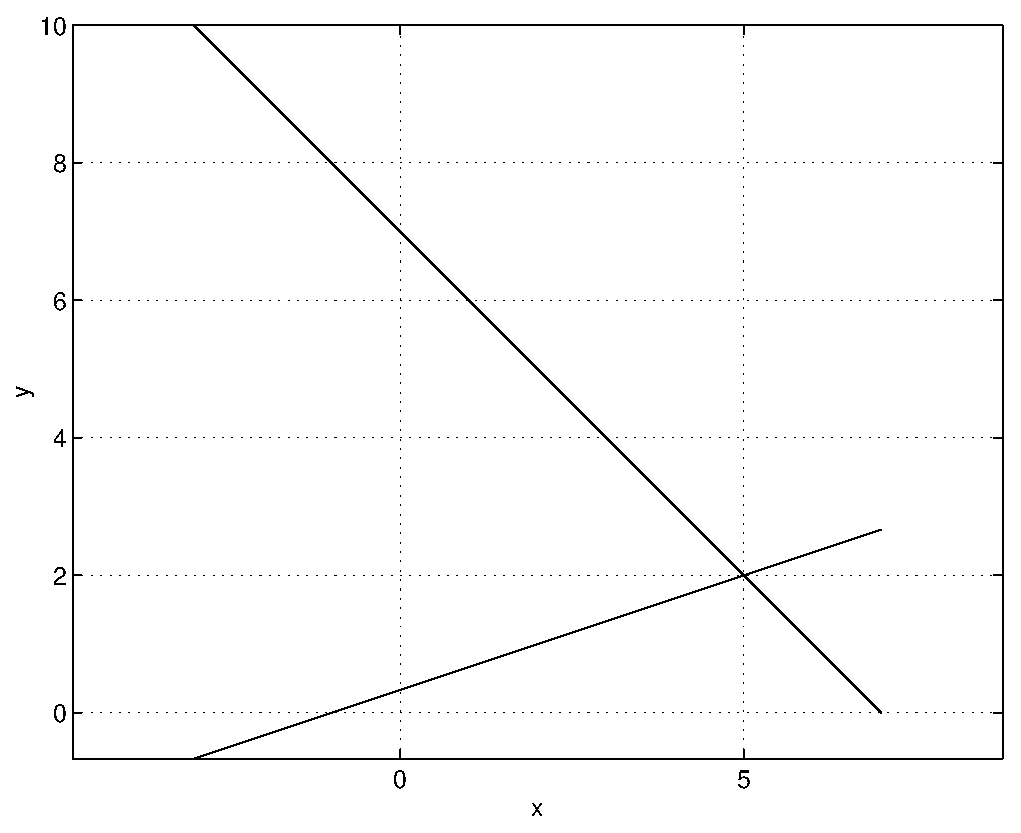
\psfig{file=figures/lineint.eps,width=3.5in}}
                       \caption{Graph of equations in \protect\Ref{small}}
                       \label{lineint}
\end{figure}


There are several principles that follow from this exercise.
\begin{itemize}
\item   Solutions to a single linear equation in two variables
form a straight line.
\item Solutions to two linear equations in two unknowns lie at
the intersection of two straight lines in the plane.
\end{itemize}
It follows that the solution to two linear equations in two
variables is a single point if the lines are not parallel.  If
these lines are parallel and unequal, then there are no
solutions, as there are no points of intersection.

\subsection*{Linear Equations in Three Dimensions}

We begin by observing that the set of all solutions to a linear
equation in three variables forms a plane\index{plane}.  More
precisely, the solutions to the equation
\begin{equation} \label{abcd}
ax+by+cz=d
\end{equation}
form a plane that is perpendicular to the vector $(a,b,c)$ ---
assuming of course that the vector $(a,b,c)$ is nonzero.

This fact is most easily proved using the {\em dot product\/}.
Recall from Chapter~\ref{chap:prelim} \Ref{e:dotproduct} that
the dot product\index{dot product} is defined by
\[
X\cdot Y = x_1y_1+x_2y_2+x_3y_3,
\]
where $X=(x_1,x_2,x_3)$ and $Y=(y_1,y_2,y_3)$.  We recall from
Chapter~\ref{chap:prelim} \Ref{dotprod=0} the following important
fact concerning dot products:
\[
X\cdot Y = 0
\]
if and only if the vectors $X$ and $Y$ are perpendicular.

Suppose that $N=(a,b,c)\neq 0$.  Consider the plane that is perpendicular
to the {\em normal vector\/}\index{normal vector} $N$ and that contains the
point $X_0$.  If the point $X$ lies in that plane, then $X-X_0$ is
perpendicular to $N$; that is,
\begin{equation} \label{XX_0}
(X-X_0)\cdot N = 0.
\end{equation}
If we use the notation
\[
X=(x,y,z) \quad \mbox{ and } \quad X_0=(x_0,y_0,z_0),
\]
then \Ref{XX_0} becomes
\[
a(x-x_0)+b(y-y_0)+c(z-z_0)=0.
\]
Setting
\[
d=ax_0 + by_0 + cz_0
\]
puts equation \Ref{XX_0} into the form \Ref{abcd}.  In this way
we see that the set of solutions to a single linear equation in
three variables forms a plane.  See Figure~\ref{F:plane}.

\begin{figure}[htb]
              \centerline{%
              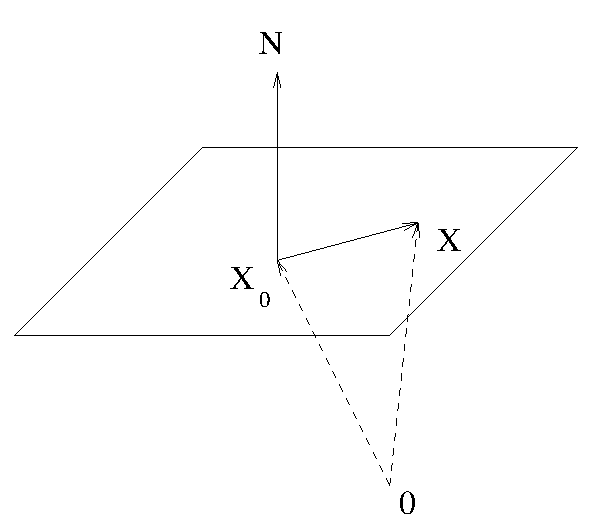
\psfig{file=figures/plane.eps,width=2.5in}}
              \caption{The plane containing $X_0$ and perpendicular to $N$.}
              \label{F:plane}
\end{figure}


We now use \Matlab to visualize the planes that are solutions to
linear equations.  Plotting an equation in three dimensions in
\Matlab follows a structure similar to the planar plots.
Suppose that we wish to plot the solutions to the equation
\begin{equation} \label{-2x+3y+z=2}
-2x+3y+z=2.
\end{equation}
We can rewrite \Ref{-2x+3y+z=2} as
\[
z=2x-3y+2.
\]
It is this function that we actually graph by typing the
commands
\begin{verbatim}
[x,y] = meshgrid(-5:0.5:5);
z = 2*x - 3*y + 2;
surf(x,y,z)
\end{verbatim} \index{\computer!meshgrid}  \index{\computer!surf}
The first command tells \Matlab to create a square grid in the
$xy$-plane.  Grid points are
equally spaced between $-5$ and $5$ at intervals of $0.5$ on
both the $x$ and $y$ axes. The second command tells \Matlab to
compute the $z$ value of the solution to \Ref{-2x+3y+z=2} at
each grid point.  The third command tells \Matlab to graph the
surface containing the points $(x,y,z)$.  See
Figure~\ref{F:p1int}.

\begin{figure}[htb]
              \centerline{%
              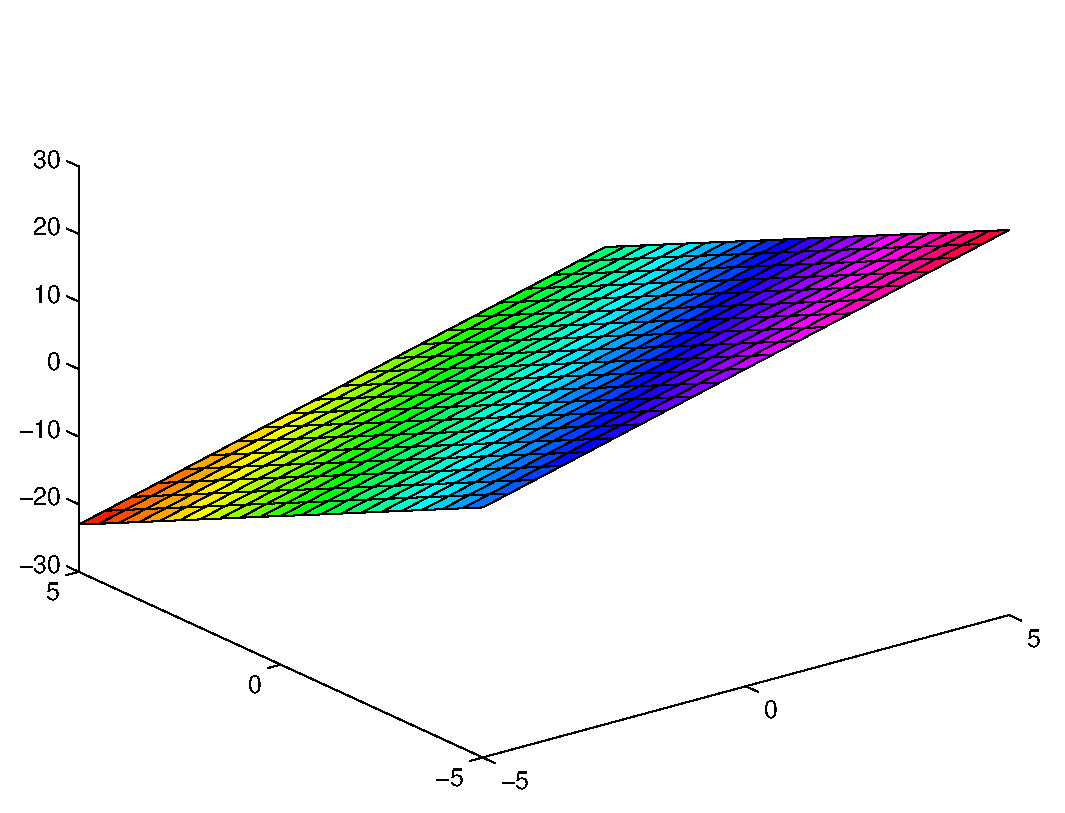
\psfig{file=figures/p1int.eps,width=3.0in}}
              \caption{Graph of \protect\Ref{-2x+3y+z=2}.}
              \label{F:p1int}
\end{figure}


We can now see that solutions to a system of two linear
equations in three unknowns consists of points that lie
simultaneously on two planes.  As long as the normal vectors to
these planes are not parallel, the intersection of the two
planes will be a line in three dimensions.  Indeed, consider the
equations
\begin{eqnarray*}
-2x + 3y + z & = & 2 \\
 2x - 3y + z & = & 0.
\end{eqnarray*}
We can graph the solution using \Matlab, as follows. We continue
from the previous graph by typing
\begin{verbatim}
hold on
z = -2*x + 3*y;
surf(x,y,z)
\end{verbatim}
The result, which illustrates that the intersection of two planes
in $\R^3$ is generally a line, is shown in Figure~\ref{F:p2int}.

\begin{figure}[htb]
              \centerline{%
              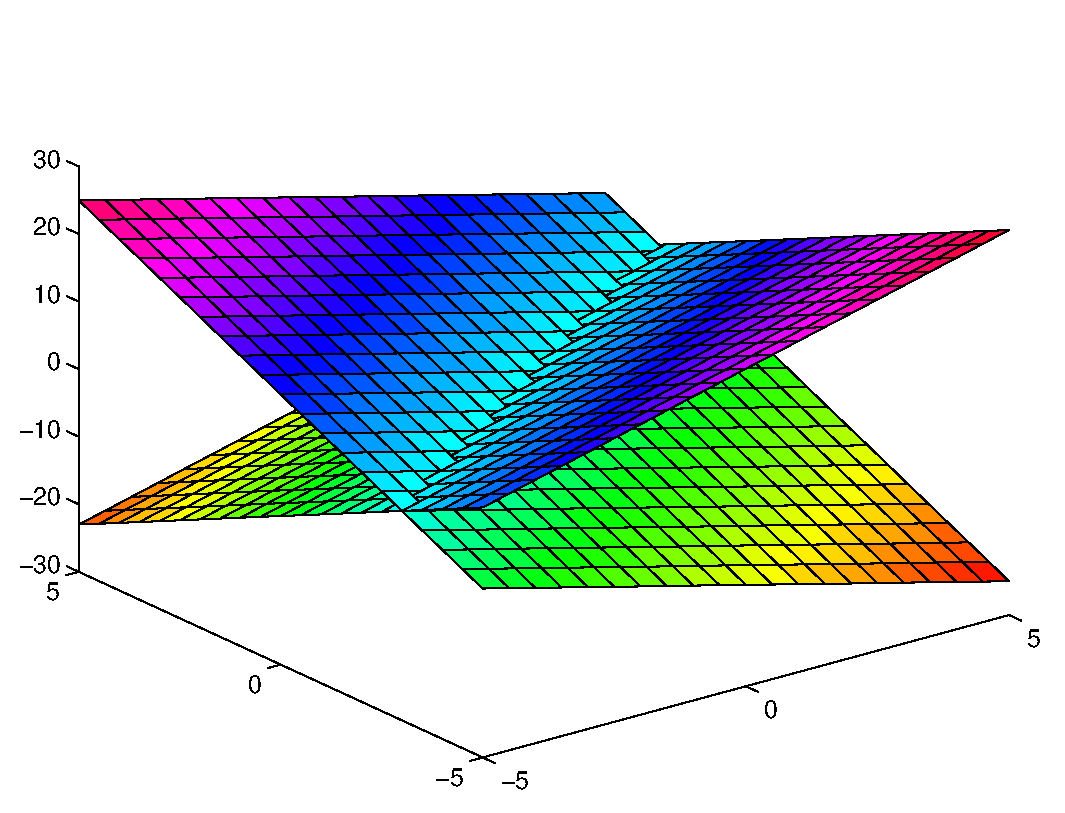
\psfig{file=figures/p2int.eps,width=3.0in}}
              \caption{Line of intersection of two planes.}
              \label{F:p2int}
\end{figure}

We can now see geometrically that the solution to three
simultaneous linear equations in three unknowns will generally
be a point --- since generally three planes in three space
intersect in a point.  To visualize this intersection, as shown in
Figure~\ref{F:p3int}, we extend the previous system of equations to
\begin{eqnarray*}
-2x +   3y + z & = & 2 \\
 2x -   3y + z & = & 0\\
-3x + 0.2y + z & = & 1.
\end{eqnarray*}
Continuing in \Matlab type
\begin{verbatim}
z = 3*x - 0.2*y + 1;
surf(x,y,z)
\end{verbatim}

\begin{figure}[htb]
              \centerline{%
              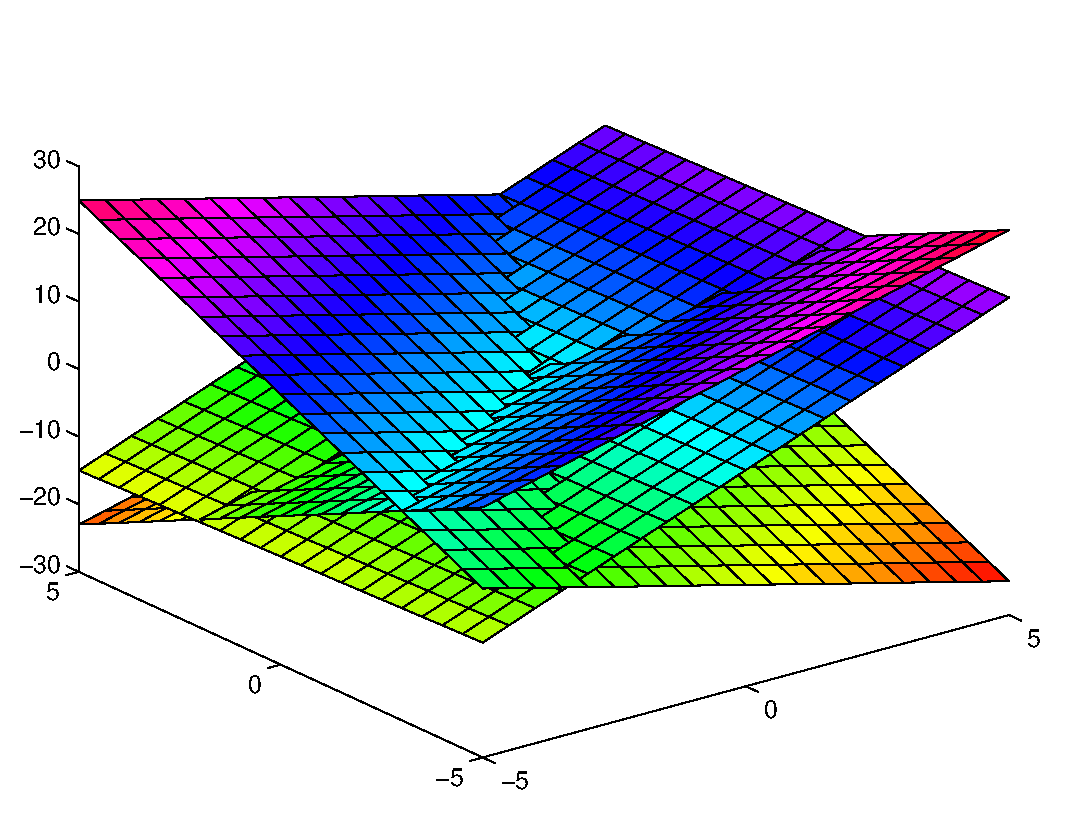
\psfig{file=figures/p3int.eps,width=3.0in}}
              \caption{Point of intersection of three planes.}
              \label{F:p3int}
\end{figure}

Unfortunately, visualizing the point of intersection of these
planes geometrically does not really help to get an accurate
numerical value of the coordinates of this intersection point.  
However, we can use \Matlab to solve this system accurately.
Denote the $3\times 3$ matrix of coefficients by {\tt A}, the 
vector of coefficients on the right hand side by {\tt b}, and 
the solution by {\tt x}.  Solve the system in \Matlab by typing
\begin{verbatim}
A = [ -2 3 1; 2 -3 1; -3 0.2 1];
b = [2; 0; 1];
x = A\b
\end{verbatim}
The point of intersection of the three planes is at
\begin{verbatim}
x =
    0.0233
    0.3488
    1.0000
\end{verbatim}

Three planes in three dimensional space need not intersect in a
single point.  For example, if two of the planes are parallel
they need not intersect at all.  The normal vectors must point
in {\em independent\/} directions to
guarantee that the intersection is a point.  Understanding the
notion of independence (it is more complicated than just not
being parallel) is part of the subject of linear algebra.
\Matlab returns ``{\tt Inf}'', which we have seen previously,
when these normal vectors are (approximately) dependent. For
example, consider Exercise~\ref{c2.2.10}.

\subsection*{Plotting Nonlinear Functions in \Matlab}

Suppose that we want to plot the graph of a nonlinear function of
a single variable, such as
\begin{equation}  \label{E:quadex}
y = x^2 - 2x + 3
\end{equation}
on the interval $[-2,5]$ using \Matlabp.  There is a difficulty:  How
do we enter the term $x^2$?  For example, suppose that we type
\begin{verbatim}
x = linspace(-2,5);
y = x*x - 2*x + 3;
\end{verbatim}
Then \Matlab responds with
\begin{verbatim}
??? Error using ==> *
Inner matrix dimensions must agree.
\end{verbatim}
The problem is that in \Matlab the variable {\tt x} is a vector of
100 equally spaced points {\tt x(1), x(2), \ldots, x(100)}.  What we
really need is a vector consisting of entries {\tt x(1)*x(1), x(2)*x(2),
\ldots, x(100)*x(100)}.  \Matlab has the facility to perform this
operation automatically and the syntax for the operation is {\tt .*}
rather than {\tt *}.  So typing
\begin{verbatim}
x = linspace(-2,5);
y = x.*x - 2*x + 3;
plot(x,y)
\end{verbatim}\index{\computer!{\tt .*}}
produces the graph of \Ref{E:quadex} in Figure~\ref{F:quadex}.
\begin{figure}[htb]
              \centerline{%
              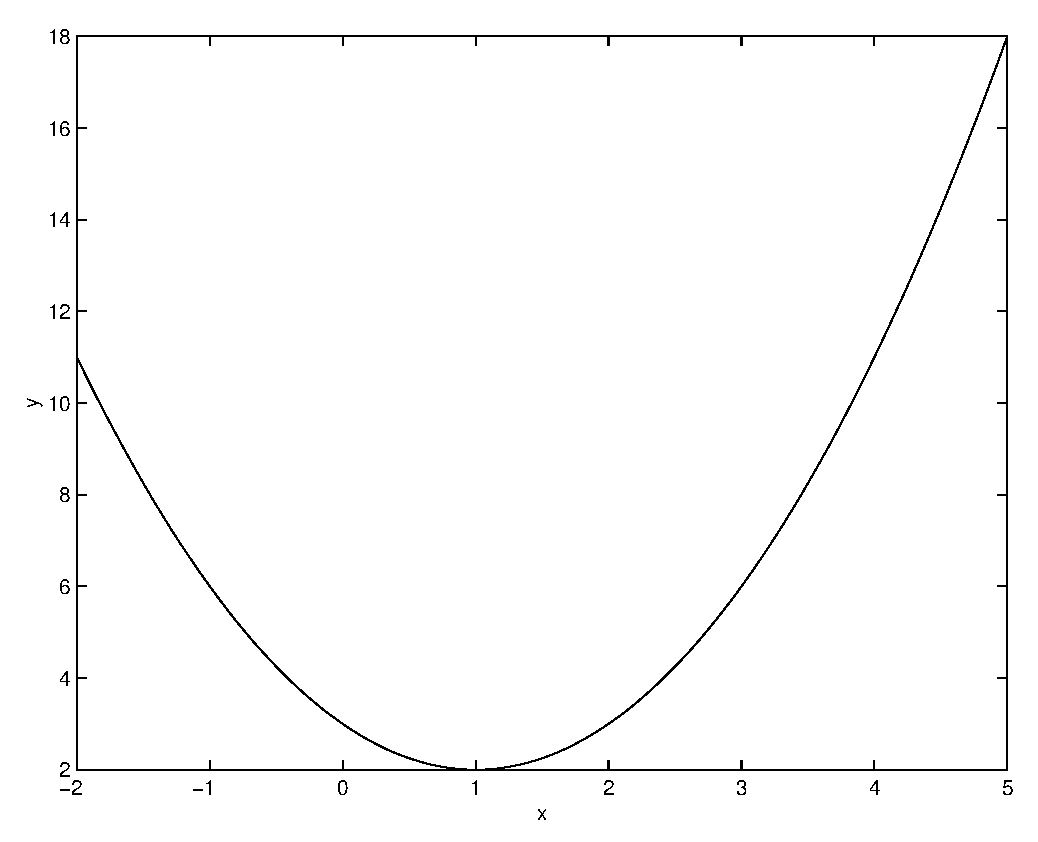
\psfig{file=figures/quadex.eps,width=3.0in}}
              \caption{Graph of $y = x^2 - 2x + 3$.}
              \label{F:quadex}
\end{figure}
In a similar fashion, \Matlab has the `dot' operations of
{\tt ./}\index{\computer!{\tt ./}},
{\tt .$\backslash$}, and  .\^{}\index{\computer!.\^{}}, as well
as {\tt .*}.

\EXER



\TEXER

\begin{exercise} \label{c2.2.5}
Find the equation for the plane perpendicular to the vector $(2,3,1)$
and containing the point $(-1,-2,3)$.
\end{exercise}

\begin{exercise} \label{c2.2.6}
Determine three systems of two linear equations in two unknowns
so that the first system has a unique solution, the second
system has an infinite number of solutions, and the third system
has no solutions.
\end{exercise}

\begin{exercise} \label{c2.2.7}
Write the equation of the plane through the origin containing the
vectors $(1,0,1)$ and $(2,-1,2)$.
\end{exercise}

\begin{exercise} \label{c2.2.8}
Find a system of two linear equations in three
unknowns whose solution set is the line consisting of scalar
multiples of the vector $(1,2,1)$.
\end{exercise}

\begin{exercise} \label{c2.2.9}
\begin{itemize}
\item[(a)] Find a vector $u$ normal to the plane $2x+2y+z=3$.
\item[(b)] Find a vector $v$ normal to the plane $x+y+2z=4$.
\item[(c)] Find the cosine of the angle between the vectors $u$ and $v$.
Use \Matlab to find the angle in degrees.
\end{itemize}
\end{exercise}

\begin{exercise} \label{c2.2.10}
Determine graphically the geometry of the set of solutions to the
system of equations in the three unknowns $x,y,z$:
\[
\begin{array}{rcrcr}
  x & + & 3z  & = & 1\\
 3x & - &  z  & = & 1\\
    &   &  z  & = & 2
\end{array}
\]
by sketching the plane of solutions for each equation individually.
Describe in words why there are no solutions to this system.
(Use \Matlab graphics to verify your sketch.  Note that you should
enter the last equation as {\tt z = 2 - 0*x - 0*y} and the first two
equations with {\tt 0*y} terms.  Try different views --- but include
{\tt view([0 1 0])} as one view.)
\end{exercise}

\CEXER

\begin{exercise} \label{c2.2.1}
Use \Matlab to solve graphically the planar system of linear
equations
\[
\arraycolsep 2pt
\begin{array}{rcrcr}
 x & + & 4y & = & -4 \\
4x & + & 3y & = &  4
\end{array}
\]
to an accuracy of two decimal points.

{\bf Hint:} The \Matlab command {\tt zoom on}\index{\computer!zoom}
allows us to
view the plot in a window whose axes are one-half those of
original.  Each time you click with the mouse on a point,
the axes' limits are halved and centered at the designated
point. Coupling {\tt zoom on} with {\tt grid on} allows you
to determine approximate numerical values for the intersection
point.
\end{exercise}

\begin{exercise} \label{c2.2.2}
Use \Matlab to solve graphically the planar system of linear
equations
\[
\arraycolsep 2pt
\begin{array}{rcrcr}
4.23x & + & 0.023y & = & -1.1 \\
1.65x & - & 2.81y & = &  1.63
\end{array}
\]
to an accuracy of two decimal points.
\end{exercise}


\begin{exercise} \label{c2.2.3}
Use \Matlab to find an approximate graphical solution to the
three dimensional system of linear equations
\[
\begin{array}{rcrcrcr}
 3x & - & 4y & + & 2z  & = & -11\\
 2x & + & 2y & + &  z  & = &   7\\
 -x & + &  y & - & 5z  & = &   7.
\end{array}
\]
Then use \Matlab to find an exact solution.
\end{exercise}


\begin{exercise} \label{c2.2.4}
Use \Matlab to determine graphically the geometry of the set of
solutions to the system of equations:
\[
\begin{array}{rcrcrcr}
  x & + & 3y & + & 4z  & = & 5\\
 2x & + &  y & + &  z  & = & 1\\
-4x & + & 3y & + & 5z  & = & 7.
\end{array}
\]
Attempt to use \Matlab to find an exact solution to this system
and discuss the implications of your calculations.

{\bf Hint:} After setting up the graphics display in \Matlabp,
you can use the command {\tt view([0,1,0])} \index{\computer!view} to get
a better view of the solution point.
\end{exercise}

\begin{exercise} \label{c2.2.a5}
Use \Matlab to graph the function $y = 2 - x\sin(x^2-1)$ on the interval
$[-2,3]$.  How many relative maxima does this function have on this interval?
\end{exercise}


\section{Gaussian Elimination}  \label{S:Gauss}

A general system of $m$ {\em linear\/} equations \index{linear}
in $n$ unknowns has the form
\begin{equation}    \label{general}
\arraycolsep 2pt
\begin{array}{rcrcrcrcrl}
 a_{11}x_1 & + & a_{12}x_2 & + & \cdots & + & a_{1n}x_n & = &   b_1
& \\
 a_{21}x_1 & + & a_{22}x_2 & + & \cdots & + & a_{2n}x_n & = &   b_2
& \\
        & \vdots &      & \vdots &    & \vdots &     & \vdots &
  & \\
 a_{m1}x_1 & + & a_{m2}x_2 & + & \cdots & + & a_{mn}x_n & = &   b_m
& .
\end{array}
\end{equation}
The entries $a_{ij}$ and $b_i$ are constants.  Our task is to find
a method for solving \Ref{general} for the variables
$x_1,\ldots,x_n$.

\subsection*{Easily Solved Equations}

Some systems are easily solved.  The system of three
equations ($m=3$) in three unknowns ($n=3$)
\begin{equation}
\begin{array}{rcrcrcrl} \label{examp3}
  x_1 & + & 2x_2 & + & 3x_3 & = &  10  & \\
      &   &  x_2 & - & \frac{1}{5}x_3 & = & \frac{7}{5}  & \\
      &   &      &   &  x_3 & = &   3  & \\
\end{array}
\end{equation}
is one example.  The $3^{rd}$ equation states that $x_3=3$.
Substituting this value into the $2^{nd}$ equation allows us to
solve the $2^{nd}$ equation for $x_2=2$.  Finally, substituting
$x_2=2$ and $x_3=3$ into the $1^{st}$ equation allows us to
solve for $x_1=-3$.  The process that we have just described is
called {\em back substitution\/}.\index{back substitution}

Next, consider the system of two equations ($m=2$) in three
unknowns ($n=3$):
\begin{equation}  \label{e23}
\begin{array}{rcrcrcrl}
  x_1 & + & 2x_2 & + & 3x_3 & = &  10  & \\
      &   &      &   &  x_3 & = &   3  & \! . \\
\end{array}
\end{equation}
The $2^{nd}$ equation in \Ref{e23} states that $x_3=3$.
Substituting
this value into the $1^{st}$ equation leads to the equation
\[
x_1 = 1-2x_2.
\]
We have shown that every solution to \Ref{e23} has the form
$(x_1,x_2,x_3)=(1-2x_2,x_2,3)$ and that every vector
$(1-2x_2,x_2,3)$ is a solution of \Ref{e23}.  Thus, there is an
infinite number of solutions to \Ref{e23}, and these solutions
can be parameterized by one number $x_2$.

\subsection*{Equations Having No Solutions}

Note that the system of equations
\begin{eqnarray*}
x_1 - x_2 = 1\\
x_1 - x_2 = 2
\end{eqnarray*}
has no solutions.

\begin{Def}
A linear system of equations is {\em inconsistent\/} if the
system has no solutions and {\em consistent\/} if the system
does have solutions.
\end{Def} \index{consistent} \index{inconsistent}

As discussed in the previous section, \Ref{incon} is an example
of a linear system that \Matlab cannot solve.  In fact, that
system is inconsistent --- inspect the $2^{nd}$ and $4^{th}$
equations in \Ref{incon}.

Gaussian elimination is an algorithm for finding all solutions
to a system of linear equations by reducing the given system to
ones like \Ref{examp3} and \Ref{e23}, that are easily solved by
back substitution.  Consequently, Gaussian elimination can also be
used to determine whether a system is consistent or inconsistent.

\subsection*{Elementary Equation Operations}

There are three ways to change a system of equations without
changing the set of solutions; Gaussian elimination
\index{Gaussian elimination} is based on this observation.  The
three elementary operations are:
\begin{enumerate}
\item   Swap two equations.
\item   Multiply a single equation by a nonzero number.
\item   Add a scalar multiple of one equation to another.
\end{enumerate}

We begin with an example:
\begin{equation}
\begin{array}{rcrcrcrl}
  x_1 & + & 2x_2 & + & 3x_3 & = &  10  & \\
  x_1 & + & 2x_2 & + &  x_3 & = &   4  & \\
 2x_1 & + & 9x_2 & + & 5x_3 & = &  27  & .\\
\end{array}
\end{equation}
Gaussian elimination works by eliminating variables from the
equations in a fashion similar to the substitution method in the
previous section.  To begin, eliminate the variable $x_1$ from
all but the $1^{st}$ equation, as follows.  Subtract the
$1^{st}$ equation from the $2^{nd}$, and subtract twice the
$1^{st}$ equation from the $3^{rd}$, obtaining:
\begin{equation}
\begin{array}{rcrcrcrl}
  x_1 & + & 2x_2 & + & 3x_3 & = &  10  & \\
      &   &      &   &-2x_3 & = &  -6  & \\
      &   & 5x_2 & - &  x_3 & = &   7  & .\\
\end{array}
\end{equation}
Next, swap the $2^{nd}$ and $3^{rd}$ equations, so that
the coefficient of $x_2$ in the new $2^{nd}$ equation is nonzero.
This yields
\begin{equation}
\begin{array}{rcrcrcrl}
  x_1 & + & 2x_2 & + & 3x_3 & = &  10  & \\
      &   & 5x_2 & - &  x_3 & = &   7  & \\
      &   &      &   &-2x_3 & = &  -6  & .\\
\end{array}
\end{equation}
Now, divide the $2^{nd}$ equation by $5$ and the $3^{rd}$
equation by $-2$ to obtain a system of equations identical to
our first example \Ref{examp3}, which we solved by back
substitution.


\subsection*{Augmented Matrices}

The process of performing Gaussian elimination when the number
of equations is greater than two or three is painful.  The
computer, however, can help with the manipulations.  We begin by
introducing the {\em augmented matrix\/}. \index{matrix!augmented}
The augmented matrix associated with \Ref{general} has
$m$ rows and $n+1$ columns and is written as:
\begin{equation}  \label{augmented}
\left(
\begin{array}{rrrr|r}
 a_{11} & a_{12} & \cdots & a_{1n} &  b_1 \\
 a_{21} & a_{22} & \cdots & a_{2n} &  b_2 \\
 \vdots & \vdots &        & \vdots & \vdots \\
 a_{m1} & a_{m2} & \cdots & a_{mn} &  b_m
\end{array}
\right)
\end{equation}
The augmented matrix contains all of the information that is
needed to solve system \Ref{general}.

\subsection*{Elementary Row Operations} \index{elementary row
operations}

The elementary operations used in Gaussian elimination
can be interpreted as {\em row operations\/} on
the augmented matrix, as follows:
\begin{enumerate}
\item   Swap two rows.
\item   Multiply a single row by a nonzero number.
\item   Add a scalar multiple of one row to another.
\end{enumerate}
We claim that by using these elementary row operations
intelligently, we can always solve a consistent linear system
--- indeed, we can determine when a linear system is consistent
or inconsistent.  The idea is to perform elementary row
operations in such a way that the new augmented matrix has zero
entries below the diagonal.

We describe this process inductively.  Begin with the $1^{st}$
column.  We assume for now that some entry in this column is
nonzero.  If $a_{11}=0$, then swap two rows so that the
number $a_{11}$ is nonzero.  Then divide the $1^{st}$ row by
$a_{11}$ so that the leading entry in that row is $1$.  Now
subtract $a_{i1}$ times the $1^{st}$ row from the $i^{th}$ row
for each row $i$ from $2$ to $m$.  The end result is that the
$1^{st}$ column has a $1$ in the $1^{st}$ row and a $0$ in every
row below the $1^{st}$.  The result is
\[
\left(\begin{array}{cccc}  1 & * & \cdots & * \\
0 & * & \cdots & * \\ \vdots & \vdots & \vdots & \vdots \\
0 & * & \cdots & * \end{array} \right).
\]


Next we consider the $2^{nd}$ column.  We assume that some entry
in that column below the $1^{st}$ row is nonzero.  So, if
necessary, we can swap two rows below the $1^{st}$ row so
that the entry $a_{22}$ is nonzero.  Then we divide the $2^{nd}$
row by $a_{22}$ so that its leading nonzero entry is $1$.  Then
we subtract appropriate multiples of the $2^{nd}$ row from each
row below the $2^{nd}$ so that all the entries in the $2^{nd}$
column below the $2^{nd}$ row are $0$.  The result is
\[
\left(\begin{array}{cccc}  1 & * & \cdots & * \\
0 & 1 & \cdots & * \\ \vdots & \vdots & \vdots & \vdots \\
0 & 0 & \cdots & * \end{array} \right).
\]

Then we continue with the $3^{rd}$ column.  That's the idea.  However,
does this process always work and what happens if all of the entries
in a column are zero?  Before answering these questions we do
experimentation with \Matlabp.

\subsection*{Row Operations in \Matlab}\index{elementary row
operations!in \protect\Matlab}

In \Matlab the $i^{th}$ row of a matrix {\tt A} is specified by
{\tt A(i,:)}.  Thus to replace the $5^{th}$ row of a matrix {\tt
A} by twice itself, we need only type:
\begin{verbatim}
A(5,:) = 2*A(5,:)
\end{verbatim}
In general, we can replace the $i^{th}$ row of the matrix
{\tt A} by $c$ times itself by typing
\begin{verbatim}
A(i,:) = c*A(i,:)
\end{verbatim}
Similarly, we can divide the $i^{th}$ row of the matrix {\tt A}
by the nonzero number $c$ by typing
\begin{verbatim}
A(i,:) = A(i,:)/c
\end{verbatim}

The third elementary row operation is performed similarly.
Suppose we want to add $c$ times the $i^{th}$ row to the
$j^{th}$ row, then we type
\begin{verbatim}
A(j,:) = A(j,:) + c*A(i,:)
\end{verbatim}
For example, subtracting $3$ times the $7^{th}$ row from the
$4^{th}$ row of the matrix {\tt A} is accomplished by typing:
\begin{verbatim}
A(4,:) = A(4,:) - 3*A(7,:)
\end{verbatim}

The first elementary row operation, swapping two rows, requires
a different kind of \Matlab command.  In \Matlabp, the $i^{th}$
and $j^{th}$ rows of the matrix {\tt A} are permuted by the
command
\begin{verbatim}
A([i j],:) = A([j i],:)
\end{verbatim}
So, to swap the $1^{st}$ and $3^{rd}$ rows of the matrix
{\tt A}, we type
\begin{verbatim}
A([1 3],:) = A([3 1],:)
\end{verbatim}  \index{\computer!A([1 3],:)}

\subsection*{Examples of Row Reduction in \Matlab}

Let us see how the row operations can be used in \Matlabp.  As
an example, we consider the augmented matrix
\begin{equation*}  \label{examp4}
\left(
\begin{array}{rrrr|r}
 1  &  3  &  0  & -1  &  -8\\
 2  &  6  & -4  &  4  &   4\\
 1  &  0  & -1  & -9  & -35\\
 0  &  1  &  0  &  3  &  10
\end{array}
\right)
\end{equation*}

We enter this information into \Matlab by typing
\begin{verbatim}
e2_3_8
\end{verbatim}
which produces the result
\begin{verbatim}
A =
     1     3     0    -1    -8
     2     6    -4     4     4
     1     0    -1    -9   -35
     0     1     0     3    10
\end{verbatim}

We now perform Gaussian elimination on {\tt A}, and then solve the 
resulting system by back substitution.  Gaussian elimination uses 
elementary row operations to set the entries that are in the lower 
left part of {\tt A} to zero. These entries are indicated by
numbers in the following matrix:
\begin{verbatim}
    *     *     *     *     *
    2     *     *     *     *
    1     0     *     *     *
    0     1     0     *     *
\end{verbatim}

Gaussian elimination \index{Gaussian elimination} works
inductively.  Since the first entry in the matrix $A$ is equal
to $1$, the first step in Gaussian elimination is to set to zero
all entries in the $1^{st}$ column below the $1^{st}$ row.  We
begin by eliminating the {\tt 2} that is the first entry in the
$2^{nd}$ row of {\tt A}.  We replace the $2^{nd}$ row by the
$2^{nd}$ row minus twice the $1^{st}$ row.  To accomplish this
elementary row operation, we type
\begin{verbatim}
A(2,:) = A(2,:) - 2*A(1,:)
\end{verbatim}
and the result is
\begin{verbatim}
A =
     1     3     0    -1    -8
     0     0    -4     6    20
     1     0    -1    -9   -35
     0     1     0     3    10
\end{verbatim}
In the next step, we eliminate the {\tt 1} from the entry in the
$3^{rd}$ row, $1^{st}$ column of {\tt A}.  We do this by
typing
\begin{verbatim}
A(3,:) = A(3,:) - A(1,:)
\end{verbatim}
which yields
\begin{verbatim}
A =
     1     3     0    -1    -8
     0     0    -4     6    20
     0    -3    -1    -8   -27
     0     1     0     3    10
\end{verbatim}

Using elementary row operations, we have now set the entries
in the $1^{st}$ column below the $1^{st}$ row to $0$.  Next,
we alter the $2^{nd}$ column.  We begin by swapping
the $2^{nd}$ and $4^{th}$ rows so that the leading nonzero entry
in the $2^{nd}$ row is $1$.   To accomplish this swap, we type
\begin{verbatim}
A([2 4],:) = A([4 2],:)
\end{verbatim}
and obtain
\begin{verbatim}
A =
     1     3     0    -1    -8
     0     1     0     3    10
     0    -3    -1    -8   -27
     0     0    -4     6    20
\end{verbatim}
The next elementary row operation is the command
\begin{verbatim}
A(3,:) = A(3,:) + 3*A(2,:)
\end{verbatim}
which leads to
\begin{verbatim}
A =
     1     3     0    -1    -8
     0     1     0     3    10
     0     0    -1     1     3
     0     0    -4     6    20
\end{verbatim}
Now we have set all entries in the $2^{nd}$ column below
the $2^{nd}$ row to $0$.

Next, we set the first nonzero entry in the $3^{rd}$ row to {\tt 1}
by multiplying the $3^{rd}$ row by $-1$, obtaining
\begin{verbatim}
A =
     1     3     0    -1    -8
     0     1     0     3    10
     0     0     1    -1    -3
     0     0    -4     6    20
\end{verbatim}

Since the leading nonzero entry in the $3^{rd}$ row is $1$,  we
next eliminate the nonzero entry in the $3^{rd}$ column,
$4^{th}$ row. This is accomplished by the following \Matlab
command:
\begin{verbatim}
A(4,:) = A(4,:) + 4*A(3,:)
\end{verbatim}
Finally, divide the $4^{th}$ row by $2$ to obtain:
\begin{verbatim}
A =
     1     3     0    -1    -8
     0     1     0     3    10
     0     0     1    -1    -3
     0     0     0     1     4
\end{verbatim}

By using elementary row operations, we have arrived at the system
\begin{equation}
\arraycolsep 2pt
\begin{array}{rcrcrcrcrl}
  x_1 & + & 3x_2 &   &     & - &  x_4 & = &  -8 & \\
      &   &  x_2 &   &     & + & 3x_4 & = &  10 & \\
      &   &      &   & x_3 & - &  x_4 & = &  -3 & \\
      &   &      &   &     &   &  x_4 & = &   4 &\! ,
\end{array}
\end{equation}
that can now be solved by back substitution.  We obtain
\begin{equation} \label{ans1}
        x_4 = 4,\quad x_3 = 1,\quad x_2 = -2,\quad x_1 = 2.
\end{equation}
We return to the original set of equations corresponding to
\Ref{examp4}
\begin{equation*}    \label{examp4_con}
\arraycolsep 2pt
\begin{array}{rcrcrcrcrl}
  x_1 & + & 3x_2 &   &      & - &  x_4 & = &  -8  & \\
 2x_1 & + & 6x_2 & - & 4x_3 & + & 4x_4 & = &   4  & \\
  x_1 &   &      & - &  x_3 & - & 9x_4 & = & -35  & \\
      &   &  x_2 &   &      & + & 3x_4 & = &  10  & \! .
\end{array}
\end{equation*}
Load the corresponding linear system into \Matlab by typing
\begin{verbatim}
e2_3_11
\end{verbatim}
The information in \Ref{examp4_con} is contained in the
coefficient matrix {\tt C} and the right hand side {\tt b}.
A direct solution is found by typing
\begin{verbatim}
x = C\b
\end{verbatim}
which yields the same answer as in \Ref{ans1}, namely,
\begin{verbatim}
x =
    2.0000
   -2.0000
    1.0000
    4.0000
\end{verbatim}

\subsection*{Introduction to Echelon Form} \index{echelon form}

Next, we discuss how Gaussian elimination works in an example
in which the number of rows and the number of columns in the
coefficient matrix are unequal.  We consider the augmented
matrix\index{matrix!augmented}
\begin{equation*}  \label{examp5}
\left(
\begin{array}{rrrrrr|r}
 1  &  0  & -2  &  3  &  4  &  0  &  1\\
 0  &  1  &  2  &  4  &  0  & -2  &  0\\
 2  & -1  & -4  &  0  & -2  &  8  & -4\\
-3  &  0  &  6  & -8  &-12  &  2  & -2
\end{array}
\right)
\end{equation*}
This information is entered into \Matlab by typing
\begin{verbatim}
e2_3_12
\end{verbatim}
Again, the augmented matrix is denoted by {\tt A}.

We begin by eliminating the {\tt 2} in the entry in the $3^{rd}$
row, $1^{st}$ column.  To accomplish the corresponding
elementary row operation, we type
\begin{verbatim}
A(3,:) = A(3,:) - 2*A(1,:)
\end{verbatim}
resulting in
\begin{verbatim}
A =
     1     0    -2     3     4     0     1
     0     1     2     4     0    -2     0
     0    -1     0    -6   -10     8    -6
    -3     0     6    -8   -12     2    -2
\end{verbatim}
We proceed with
\begin{verbatim}
A(4,:) = A(4,:) + 3*A(1,:)
\end{verbatim}
to create two more zeros in the $4^{th}$ row.  Finally, we
eliminate the {\tt -1} in the $3^{rd}$ row, $2^{nd}$
column by
\begin{verbatim}
A(3,:) = A(3,:) + A(2,:)
\end{verbatim}
to arrive at
\begin{verbatim}
A =
     1     0    -2     3     4     0     1
     0     1     2     4     0    -2     0
     0     0     2    -2   -10     6    -6
     0     0     0     1     0     2     1
\end{verbatim}
Next we set the leading nonzero entry in the $3^{rd}$ row to $1$
by dividing the $3^{rd}$ row by $2$.   That is, we type
\begin{verbatim}
A(3,:) = A(3,:)/2
\end{verbatim}
to obtain
\begin{verbatim}
A =
     1     0    -2     3     4     0     1
     0     1     2     4     0    -2     0
     0     0     1    -1    -5     3    -3
     0     0     0     1     0     2     1
\end{verbatim}
We say that the matrix {\tt A} is in (row) {\em echelon form\/}
\index{echelon form} since the first nonzero entry in each row
is a {\tt 1}, each entry in a column below a leading {\tt 1} is
{\tt 0}, and the leading {\tt 1} moves to the right as you go
down the matrix.  In row echelon form, the entries where leading
$1$'s occur are called {\em pivots\/}.\index{pivot}

If we compare the structure of this matrix to the ones we have
obtained previously, then we see that here we have two columns
too many.  Indeed, we may solve these equations by back
substitution for any choice of the variables $x_5$ and $x_6$.

The idea behind back substitution \index{back substitution} is
to solve the last equation for the variable corresponding to the
first nonzero coefficient.  In this case, we use the $4^{th}$
equation to solve for $x_4$ in terms of $x_5$ and $x_6$, and
then we substitute for $x_4$ in the first three equations.  This
process can also be accomplished by elementary row operations.
Indeed, eliminating the variable $x_4$ from the first three
equations is the same as using row operations to set the first
three entries in the $4^{th}$ column to {\tt 0}.  We can do this
by typing
\begin{verbatim}
A(3,:) = A(3,:) + A(4,:);
A(2,:) = A(2,:) - 4*A(4,:);
A(1,:) = A(1,:) - 3*A(4,:)
\end{verbatim}
{\bf Remember:} By typing semicolons after the first two rows, we
have told \Matlab not to print the intermediate results.  Since
we have not typed a semicolon after the $3^{rd}$ row, \Matlab
outputs
\begin{verbatim}
A =
     1     0    -2     0     4    -6    -2
     0     1     2     0     0   -10    -4
     0     0     1     0    -5     5    -2
     0     0     0     1     0     2     1
\end{verbatim}
We proceed with back substitution by eliminating the nonzero
entries in the first two rows of the $3^{rd}$ column.  To do
this, type
\begin{verbatim}
A(2,:) = A(2,:) - 2*A(3,:);
A(1,:) = A(1,:) + 2*A(3,:)
\end{verbatim}
which yields
\begin{verbatim}
A =
     1     0     0     0    -6     4    -6
     0     1     0     0    10   -20     0
     0     0     1     0    -5     5    -2
     0     0     0     1     0     2     1
\end{verbatim}
The augmented matrix is now in {\em reduced echelon form}
\index{echelon form!reduced} and the corresponding system of
equations has the form
\begin{equation}   \label{e:refexamp5}
\arraycolsep 2pt
\begin{array}{rcrcrcrcrcrcrl}
  x_1 &   &     &   &     &  &     & - &  6x_5 & + &  4x_6 & = &
-6 & \\
      &   & x_2 &   &     &  &     & + & 10x_5 & - & 20x_6 & = &
0 & \\
      &   &     &   & x_3 &  &     & - &  5x_5 & + &  5x_6 & = &
-2 & \\
      &   &     &   &     &  & x_4 &   &       & + &  2x_6 & = &
1 &\! ,
\end{array}
\end{equation}
A matrix is in reduced echelon form \index{echelon form!reduced}
if it is in echelon form and if {\em every\/} entry in a column
containing a pivot, other than the pivot itself, is {\tt 0}.

Reduced echelon form allows us to solve directly this system of
equations in terms of the variables $x_5$ and $x_6$,
\begin{equation}  \label{e:refexamp6}
\left(\begin{array}{c} x_1\\x_2\\x_3\\x_4\\x_5\\x_6\end{array}\right) =
\left(\begin{array}{c} -6+6x_5-4x_6\\-10x_5+20x_6\\
-2+5x_5-5x_6\\1-2x_6\\x_5\\x_6\end{array}\right).
\end{equation}
It is important to note that every consistent system of linear equations
corresponding to an augmented matrix in reduced echelon form can be
solved as in \Ref{e:refexamp6} --- and this is one reason for emphasizing
reduced echelon form.  We will discuss the reduction to reduced echelon
form in more detail in the next section.

\EXER


\TEXER

\noindent In Exercises~\ref{c2.3.6a} -- \ref{c2.3.6c} determine
whether the given matrix is in reduced echelon form.
\begin{exercise} \label{c2.3.6a}
$\left(\begin{array}{rrrr}
1 & -1 &  0 &   1   \\
0 &  1 &  0 &  -6    \\
0 &  0 &  1 &   0   \end{array}\right)$.
\end{exercise}
\begin{exercise} \label{c2.3.6b}
$\left(\begin{array}{rrrr}
1 &  0 & -2 &   0   \\
0 &  1 &  4 &   0    \\
0 &  0 &  0 &   1  \end{array}\right)$.
\end{exercise}
\begin{exercise} \label{c2.3.6c}
$\left(\begin{array}{rrrr}
0 &  1 &  0 &   3   \\
0 &  0 &  2 &   1    \\
0 &  0 &  0 &   0   \end{array}\right)$.
\end{exercise}

\noindent In Exercises~\ref{c2.3.7a} -- \ref{c2.3.7c} we list
the reduced echelon form of an augmented matrix of a system of
linear equations.  Which columns in these augmented matrices
contain pivots?  Describe all solutions to these systems of
equations in the form of \Ref{e:refexamp6}.
\begin{exercise} \label{c2.3.7a}
$\left(\begin{array}{rrr|r}
 1  &  4 & 0 & 0\\
 0  &  0 & 1 & 5\\
 0  &  0 & 0 & 0
\end{array}\right)$.
\end{exercise}
\begin{exercise} \label{c2.3.7b}
$\left(\begin{array}{rrrr|r}
 1  &  2 & 0 & 0 & 0\\
 0  &  0 & 1 & 1 & 0\\
 0  &  0 & 0 & 0 & 1
\end{array}\right)$.
\end{exercise}
\begin{exercise} \label{c2.3.7c}
$\left(\begin{array}{rrrr|r}
 1  & -6 & 0 & 0 & 1\\
 0  &  0 & 1 & 0 & 9 \\
 0  &  0 & 0 & 0 & 0
\end{array}\right)$.
\end{exercise}


\begin{exercise} \label{c2.3.8}
(a) Consider the $2\times 2$ matrix
\begin{equation}  \label{e:2x2}
\mattwo{a}{b}{c}{1}
\end{equation}
where $a,b,c\in\R$ and $a\neq 0$.  Show that \Ref{e:2x2}
is row equivalent to the matrix
\[
\left(\begin{array}{cc} 1 & \frac{b}{a} \\ 0 & \frac{a-bc}{a}
\end{array} \right).
\]
(b)  Show that \Ref{e:2x2} is row equivalent to the
identity matrix if and only if $a\neq bc$.
\end{exercise}

\begin{exercise} \label{c2.3.9}
Use row reduction and back substitution to solve the following
system of two equations in three unknowns:
\[
\begin{array}{rcrcrcrc}
 x_1 & - & x_2 & + & x_3 & = & 1 \\
2x_1 & + & x_2 & - & x_3 & = & -1
\end{array}
\]
Is $(1,2,2)$ a solution to this system?  If not, is there a
solution for which $x_3=2$?
\end{exercise}

\noindent In Exercises~\ref{c2.3.10a} -- \ref{c2.3.10b} determine the
augmented matrix and all solutions for each system of linear equations
\begin{exercise} \label{c2.3.10a}
$\begin{array}{rcl}
x-y+z & = & 1 \\
4x+y+z & = & 5 \\
2x+3y-z & = & 2 \end{array}$.
\end{exercise}
\begin{exercise} \label{c2.3.10b}
$\begin{array}{rcl}
2x-y+z+w & = & 1\\
x+2y-z+w & = & 7 \end{array}$.
\end{exercise}

\noindent In Exercises~\ref{c2.3.11a} -- \ref{c2.3.11d} consider the
augmented matrices representing systems of linear equations, and decide
\begin{itemize}
\item[(a)] if there are zero, one or infinitely many solutions, and
\item[(b)] if solutions are not unique, how many variables can be
assigned arbitrary values.
\end{itemize}
\begin{exercise} \label{c2.3.11a}
$\left(\begin{array}{ccc|c} 1 & 0 & 0 &3 \\0 & 2 & 1 & 1\\ 0 & 0 & 0 & 0
\end{array}\right)$.
\end{exercise}
\begin{exercise} \label{c2.3.11b}
$\left(\begin{array}{cccc|c} 1 & 2 & 0 & 0 & 3\\ 0 & 1 & 1 & 0 & 1\\
0 & 0 & 0 & 0 & 2 \end{array}\right)$.
\end{exercise}
\begin{exercise} \label{c2.3.11c}
$\left(\begin{array}{ccc|c}  1 & 0 & 2 & 1\\ 0 & 5 & 0 & 2 \\ 0 & 0 & 4 & 3
\end{array}\right)$.
\end{exercise}
\begin{exercise} \label{c2.3.11d}
$\left(\begin{array}{cccc|c} 1 & 0 & 2 & 0 & 3 \\ 2 & 3 & 6 & 1 & 16\\
0 & 3 & 2 & 1 & 10 \\ 0 & 0 & 0 & 0 & 0  \end{array}\right)$.
\end{exercise}

\noindent A system of $m$ equations in $n$ unknowns is linear if it has
the form \Ref{general}; any other system of equations is called 
{\em nonlinear\/}. \index{nonlinear}  In Exercises~\ref{c2.3.12a} -- 
\ref{c2.3.12e} decide whether each of the given systems of equations 
is linear or nonlinear.
\begin{exercise} \label{c2.3.12a}
\[
\begin{array}{rcl}
3x_1 - 2x_2 +14x_3-7x_4 & = & 35\\
2x_1 + 5x_2 - 3x_3 + 12x_4 & = & -1
\end{array}
\]
\end{exercise}
\begin{exercise} \label{c2.3.12b}
\[
\begin{array}{rcl}
3x_1 + \pi x_2  & = & 0\\
2x_1 - e x_2    & = & 1
\end{array}
\]
\end{exercise}
\begin{exercise} \label{c2.3.12c}
\[
\begin{array}{rcl}
3x_1x_2 -x_2  & = & 10\\
2x_1 -   x_2^2    & = & -5
\end{array}
\]
\end{exercise}
\begin{exercise} \label{c2.3.12d}
\[
\begin{array}{rcl}
3x_1  -x_2  & = & \cos(12)\\
2x_1 -   x_2    & = & -5
\end{array}
\]
\end{exercise}
\begin{exercise} \label{c2.3.12e}
\[
\begin{array}{rcl}
3x_1  - \sin(x_2)  & = & 12\\
2x_1 -   x_3    & = & -5
\end{array}
\]
\end{exercise}

\CEXER



\noindent In Exercises~\ref{c2.3.1a} -- \ref{c2.3.1c} use elementary row
operations and \Matlab to put each of the given matrices into row echelon
form.  Suppose that the matrix is the augmented matrix for a system of
linear equations.  Is the system consistent or inconsistent?

\begin{exercise} \label{c2.3.1a}
\[
\left(\begin{array}{rrr}
 2 &  1  &  1   \\
 4 &  2  &  3
\end{array}\right).
\]
\end{exercise}
\begin{exercise} \label{c2.3.1b}
\[
\left(\begin{array}{rrrr}
 3  & -4 & 0 & 2\\
 0  &  2 & 3 & 1\\
 3  &  1 & 4 & 5
\end{array}\right).
\]
\end{exercise}
\begin{exercise} \label{c2.3.1c}
\[
\left(\begin{array}{rrrr}
 -2 & 1 &  9 & 1\\
  3 & 3 & -4 & 2\\
  1 & 4 &  5 & 5
\end{array}\right).
\]
\end{exercise}

\noindent {\bf Observation:} {\rm In standard format \Matlab displays
all nonzero real numbers with four decimal places while it displays
zero as $0$.  An unfortunate consequence of this display is that
when a matrix has both zero and noninteger entries, the columns
will not align --- which is a nuisance.  You can work with
rational numbers rather than decimal numbers by typing {\tt
format rational}.  Then the columns will align.}

\begin{exercise} \label{c2.3.2}
Load the following $6\times 8$ matrix $A$ into \Matlab by typing
{\tt e2\_3\_16}.
\begin{equation*}
A=\left(\begin{array}{rrrrrrrr}
0 & 0 &  0 &   1 &   3 &   5 & 0 &  9 \\
0 & 3 &  6 &  -6 &  -6 & -12 & 0 &  1 \\
0 & 2 &  4 &  -5 &  -7 &  14 & 0 &  1 \\
0 & 1 &  2 &   1 &  14 &  21 & 0 & -1 \\
0 & 0 &  0 &   2 &   4 &   9 & 0 &  7 \\
0 & 5 & 10 & -11 & -13 &   2 & 0 &  2
\end{array}\right)
\end{equation*}
Use \Matlab to transform this matrix to row echelon form.
\end{exercise}

\begin{exercise} \label{c2.3.3}
Use row reduction and back substitution to solve the following
system of linear equations:
\[
\begin{array}{rcrcrcrcr}
2x_1 & + &  3x_2 &  - &  4x_3 & + &  x_4 &  = & 2 \\
3x_1 & - &   x_2 &  - &   x_3 & + & 2x_4 &  = & 4 \\
 x_1 & - &  7x_2 &  + &  5x_3 & - &  x_4 &  = & 6
\end{array}
\]
\end{exercise}


\begin{exercise} \label{c2.3.4}
{\bf Comment:} {\rm To understand the point of this exercise you
must begin by typing the \Matlab command {\tt format short e}.
This command will set a format in which you can see the
difficulties that sometimes arise in numerical computations.}

Consider the following two $3\times 3$-matrices:
\begin{equation*}
A=\left( \begin{array}{rrr}
     1  &  3  &  4\\
     2  &  1  &  1\\
    -4  &  3  &  5
\end{array}\right) \AND
B=\left( \begin{array}{rrr}
     3  &  1  &  4\\
     1  &  2  &  1\\
     3  & -4  &  5
\end{array}\right).
\end{equation*}
Note that matrix $B$ is obtained from matrix $A$ by interchanging the
first two columns.
\begin{itemize}
\item[(a)] Use \Matlab to put $A$ into row echelon form using the
transformations
\begin{enumerate}
\item Subtract $2$ times the $1^{st}$ row from the $2^{nd}$.
\item Add $4$ times the $1^{st}$ row to the $3^{rd}$.
\item Divide the $2^{nd}$ row by $-5$.
\item Subtract $15$ times the $2^{nd}$ row from the $3^{rd}$.
\end{enumerate}
\item[(b)] Put $B$ by hand into row echelon form using the
transformations
\begin{enumerate}
\item Divide the $1^{st}$ row by $3$.
\item Subtract the $1^{st}$ row from the $2^{nd}$.
\item Subtract $3$ times the $1^{st}$ row from the $3^{rd}$.
\item Multiply the $2^{nd}$ row by $3/5$.
\item Add $5$ times the $2^{nd}$ row to the $3^{rd}$.
\end{enumerate}
\item[(c)] Use \Matlab to put $B$ into row echelon form using the
same transformations as in part (b).
\item[(d)] Discuss the outcome of the three transformations.  Is
there a difference in the results?  Would you expect to see a
difference?  Could the difference be crucial when solving a system
of linear equations?
\end{itemize}
\end{exercise}

\begin{exercise} \label{c2.3.5}
Find a cubic polynomial
\[
p(x) = ax^3 + bx^2 + cx + d
\]
so that $p(1)=2$, $p(2)=3$, $p'(-1)=-1$, and $p'(3)=1$.
\end{exercise}



\section{Reduction to Echelon Form}
\label{S:2.4}

In this section, we formalize our previous numerical
experiments.  We define more precisely the notions of echelon
form and reduced echelon form matrices, and we prove that every
matrix can be put into reduced echelon form using a sequence of
elementary row operations.  Consequently, we will have developed
an algorithm for determining whether a system of linear
equations is consistent or inconsistent, and for determining all
solutions to a consistent system.

\begin{Def}
A matrix $E$ is in (row) {\em echelon form\/} \index{echelon
form} if two conditions hold.
\begin{enumerate}
\item[(a)] The first nonzero entry in each row of $E$ is equal
to $1$.  This leading entry $1$ is called a {\em pivot\/}. \index{pivot}
\item[(b)] A pivot in the $(i+1)^{st}$ row of $E$ occurs in a column to
the right of the column where the pivot in the $i^{th}$ row occurs.
\end{enumerate}
\end{Def}

Here are three examples of matrices that are in echelon form.
The pivot in each row (which is always equal to $1$) is preceded
by a $*$.
\[
\left(\begin{array}{rrrrrrr}
    *1   &  0   &  -1  &  0  &  -6  &   4  &  -6\\
     0   & *1   &  4   &  0  &   0  &  -2  &   0\\
     0   &  0   &  0   & *1  &  -5  &   5  &  -2\\
     0   &  0   &  0   &  0  &   0  &  *1  &   0
\end{array} \right)
\]
\[
\left(\begin{array}{rrrrr}
    *1 &   0  &  -1  &   0  &  -6 \\
     0 &  *1  &   0  &   3  &   0  \\
     0 &   0  &   0  &  *1  &  -5   \\
     0 &   0  &   0  &   0  &   0
\end{array} \right)
\]
\[
\left(\begin{array}{rrrrr}
     0  &  *1  &  -1  &  14  &  -6 \\
     0  &   0  &   0  &  *1  &  15  \\
     0  &   0  &   0  &   0  &   0   \\
     0  &   0  &   0  &   0  &   0
\end{array} \right)
\]
Here are three examples of matrices that are {\em not\/} in echelon form.
\[
\left(\begin{array}{rrrr}
     0  &   0  &   1  &  15  \\
     1  &  -1  &  14  &  -6 \\
     0  &   0  &   0  &   0   \\
\end{array} \right)
\AND
\left(\begin{array}{rrrr}
     1  &  -1  &  14  &  -6 \\
     0  &   0  &   3  &  15  \\
     0  &   0  &   0  &   0   \\
\end{array} \right)
\AND
\left(\begin{array}{rrrr}
     1  &  -1  &  14  &  -6 \\
     0  &   0  &   0  &   0   \\
     0  &   0  &   1  &  15  \\
\end{array} \right)
\]


\begin{Def} \label{D:roweq}\index{row!equivalent}
Two $m\times n$ matrices are {\em row equivalent\/} if one can be
transformed to the other by a sequence of elementary row
operations.
\end{Def}
\index{row!equivalent}

Let $A=(a_{ij})$ be a matrix with $m$ rows and $n$ columns.  We
want to show that we can perform row operations on $A$ so that
the transformed matrix is in echelon form; that is, $A$ is row
equivalent to a matrix in echelon form.  If $A=0$, then we
are finished.  So we assume that some entry in $A$ is nonzero
and that the $1^{st}$ column where that nonzero entry occurs is in
the $k^{th}$ column.  By swapping rows we can assume that
$a_{1k}$ is nonzero.  Next, divide the $1^{st}$ row by $a_{1k}$,
thus setting $a_{1k}=1$.  Now, using
\Matlab notation, perform the row operations
\begin{verbatim}
A(i,:) = A(i,:) - A(i,k)*A(1,:)
\end{verbatim}
for each $i\geq 2$.  This sequence of row operations leads to a
matrix whose first nonzero column has a $1$ in the $1^{st}$ row
and a zero in each row below the $1^{st}$ row.

Now we look for the next column that has a nonzero entry below
the $1^{st}$ row and call that column $\ell$.  By construction
$\ell>k$.  We can swap rows so that the entry in the $2^{nd}$
row, $\ell^{th}$ column is nonzero.  Then we divide the $2^{nd}$
row by this nonzero element, so that the pivot in the $2^{nd}$
row is $1$.  Again we perform elementary row operations so that
all entries below the $2^{nd}$ row in the $\ell^{th}$ column are
set to $0$.  Now proceed inductively until we run out of nonzero
rows.

This argument proves:
\begin{prop}  \label{P:echform}
Every matrix is row equivalent to a matrix in echelon form.
\end{prop}

More importantly, the previous argument provides an algorithm for
transforming matrices into echelon form.

\subsection*{Reduction to Reduced Echelon Form}

\begin{Def}\index{echelon form!reduced}
A matrix $E$ is in {\em reduced echelon form\/} if
\begin{enumerate}
\item[(a)]        $E$ is in echelon form, and
\item[(b)] in every column of $E$ having a pivot, every entry
in that column other than the pivot is $0$.
\end{enumerate}
\end{Def}

We can now prove
\begin{thm}  \label{T:redechform}
Every matrix is row equivalent \index{row!equivalent} to a matrix
in reduced echelon form.
\end{thm}

\proof Let $A$ be a matrix.  Proposition~\ref{P:echform} states
that we can transform $A$ by elementary row operations to a matrix
$E$ in echelon form.  Next we transform $E$ into reduced echelon
form by some additional elementary row operations, as follows.
Choose the pivot in the last nonzero row of $E$.  Call that row
$\ell$, and let $k$ be the column where the pivot occurs.  By
adding multiples of the $\ell^{th}$ row to the rows above, we can
transform each entry in the $k^{th}$ column above the pivot to $0$.
Note that none of these row operations alters the matrix before
the $k^{th}$ column.  (Also note that this process is identical to
the process of back substitution.)

Again we proceed inductively by choosing the pivot in the
$(\ell-1)^{st}$ row, which is $1$, and zeroing out all entries
above that pivot using elementary row operations.  \qed

\subsection*{Reduced Echelon Form in \Matlab}

Preprogrammed into \Matlab is a routine to row reduce any
matrix to reduced echelon form.  The command is
{\tt rref}\index{\computer!rref}.
For example, recall the $4\times 7$ matrix $A$ in \Ref{examp5}
by typing {\tt e2\_3\_12}.  Put $A$ into reduced row echelon
form by typing {\tt rref(A)} and obtaining
\begin{verbatim}
ans =
     1     0     0     0    -6     4    -6
     0     1     0     0    10   -20     0
     0     0     1     0    -5     5    -2
     0     0     0     1     0     2     1
\end{verbatim}
Compare the result with the system of equations \Ref{e:refexamp5}.

\subsection*{Solutions to Systems of Linear Equations}

Originally, we introduced elementary row
operations as operations that do not change solutions to the
linear system.  More precisely, we discussed how solutions to
the original system are still solutions to the transformed
system and how no new solutions are introduced by elementary
row operations.  This argument is most easily seen by observing
that
\begin{center}
all elementary row operations are invertible
\end{center}
--- they can be undone.

For example, swapping two rows is undone by just swapping these
rows again.  Similarly, multiplying a row by a nonzero number
$c$ is undone by just dividing that same row by $c$.  Finally,
adding $c$ times the $j^{th}$ row to the $i^{th}$ row is undone
by subtracting $c$ times the $j^{th}$ row from the $i^{th}$ row.

Thus, we can make several observations about solutions to linear
systems.  Let $E$ be an augmented matrix corresponding to a system
of linear equations having $n$ variables.  Since an augmented
matrix is formed from the matrix of coefficients by adding a
column, we see that the augmented matrix has $n+1$ columns.

\begin{thm} \label{number}
Suppose that $E$ is an $m\times(n+1)$ augmented matrix that is in 
reduced echelon form.  Let $\ell$ be the number of nonzero rows in $E$
\begin{enumerate}
\item[(a)] The system of linear equations corresponding to $E$
is inconsistent if and only if the $\ell^{th}$ row in $E$ has a
pivot in the $(n+1)^{st}$ column.
\item[(b)] If the linear system corresponding to $E$ is consistent,
then the set of all solutions is parameterized by $n-\ell$
parameters.
\end{enumerate} \index{inconsistent} \index{consistent}
\end{thm}

\proof  Suppose that the last nonzero row in $E$ has its
pivot in the $(n+1)^{st}$ column. Then the corresponding
equation is:
\[
0x_1 + 0x_2 + \cdots + 0x_n = 1,
\]
which has no solutions.  Thus the system is inconsistent.

Conversely, suppose that the last nonzero row has its pivot
before the last column.  Without loss of generality, we can
renumber the columns --- that is, we can renumber the variables
$x_j$ --- so that the pivot in the $i^{th}$ row occurs in the
$i^{th}$ column, where $1\leq i\leq\ell$.  Then the associated
system of linear equations has the form:
\begin{eqnarray*}
x_1 + a_{1,\ell+1}x_{\ell+1} + \cdots + a_{1,n}x_n & = &  b_1 \\
x_2 + a_{2,\ell+1}x_{\ell+1} + \cdots + a_{2,n}x_n & = &  b_2 \\
\vdots &   &    \vdots  \\
x_\ell + a_{\ell,\ell+1}x_{\ell+1} + \cdots + a_{\ell,n}x_n & = & b_\ell.
\end{eqnarray*}
This system can be rewritten in the form:
\begin{eqnarray}
  x_1  & = &  b_1 - a_{1,\ell+1}x_{\ell+1} - \cdots - a_{1,n}x_n
\nonumber\\
  x_2  & = &  b_2 - a_{2,\ell+1}x_{\ell+1} - \cdots - a_{2,n}x_n
\label{e1-ell}\\
\vdots &   &    \vdots \nonumber \\
x_\ell & = &  b_\ell - a_{\ell,\ell+1}x_{\ell+1} - \cdots -
a_{\ell,n}x_n.
\nonumber
\end{eqnarray}

Thus, each choice of the $n-\ell$ numbers
$x_{\ell+1},\ldots,x_n$ uniquely determines values of
$x_1,\ldots,x_\ell$ so that $x_1,\ldots,x_n$ is a solution to
this system.  In particular, the system is consistent, so (a) is
proved; and the set of all solutions is parameterized by
$n-\ell$ numbers, so (b) is proved.  \qed

\subsubsection*{Two Examples Illustrating Theorem~\ref{number}}

The reduced echelon form matrix
\[
E = \left(\begin{array}{ccc|c} 1 & 5 & 0 & 0 \\ 0 & 0 & 1 & 0\\
	0 & 0 & 0 & 1 \end{array}\right)
\]
is the augmented matrix of an inconsistent system of three equations
in three unknowns.

The reduced echelon form matrix
\[
E = \left(\begin{array}{ccc|c} 1 & 5 & 0 & 2 \\ 0 & 0 & 1 & 5\\
	0 & 0 & 0 & 0 \end{array}\right)
\]
is the augmented matrix of a consistent system of three equations
in three unknowns $x_1,x_2,x_3$.  For this matrix $n=3$ and $\ell=2$.
It follows from Theorem~\ref{number} that the solutions to this system
are specified by one parameter.  Indeed, the solutions are
\begin{eqnarray*}
x_1 & = & 2 - 5x_2\\
x_3 & = & 5
\end{eqnarray*}
and are specified by the one parameter $x_2$.


\subsubsection*{Consequences of Theorem~\ref{number}}

It follows from Theorem~\ref{number} that linear systems of equations
with fewer equations than unknowns and with zeros on the right hand
side always have nonzero solutions.  More precisely:
\begin{cor}  \label{existencehomo}
Let $A$ be an $m\times n$ matrix where $m<n$.  Then the system of
linear equations whose augmented matrix is $(A|0)$ has a nonzero
solution.
\end{cor}

\proof Perform elementary row operations on the augmented matrix $(A|0)$
to arrive at the reduced echelon form matrix $(E|0)$.  Since the zero
vector is a solution, the associated system of equations is consistent.
Now the number of nonzero rows $\ell$ in $(E|0)$ is less than or equal to
the number of rows $m$ in $E$.  By assumption $m<n$ and hence $\ell<n$.
It follows from Theorem~\ref{number} that solutions to the linear system
are parametrized by $n-\ell \ge 1$ parameters and that there are nonzero
solutions.   \qed

Recall that two $m\times n$ matrices are row equivalent if one
can be transformed to the other by elementary row operations.

\begin{cor}  \label{consistent}
Let $A$ be an $n\times n$ square matrix and let $b$ be in
$\R^n$.  Then $A$ is row equivalent to the identity matrix $I_n$
if and only if the system of linear equations whose augmented
matrix is $(A|b)$ has a unique solution.
\end{cor} \index{matrix!identity}  \index{matrix!augmented}

\proof	Suppose that $A$ is row equivalent to $I_n$.  Then, by using
the same sequence of elementary row operations, it follows that
the $n\times (n+1)$ augmented matrix $(A|b)$ is row equivalent
to $(I_n|c)$ for some vector $c\in\R^n$.  The system of linear
equations that corresponds to $(I_n|c)$ is:
\[
\begin{array}{ccc}
x_1 & = & c_1 \\
\vdots & \vdots & \vdots \\
x_n & = & c_n,
\end{array}
\]
which transparently has the unique solution $x=(c_1,\ldots,c_n)$.
Since elementary row operations do not change the solutions of
the equations, the original augmented system $(A|b)$ also has a
unique solution.

Conversely, suppose that the system of linear equations
associated to $(A|b)$ has a unique solution.  Suppose that
$(A|b)$ is row equivalent to a reduced echelon form matrix $E$.
Suppose that the last nonzero row in $E$ is the $\ell^{th}$ row.
Since the system has a solution, it is consistent.  Hence
Theorem~\ref{number}(b) implies that the solutions to the system
corresponding to $E$ are parameterized by $n-\ell$ parameters.
If $\ell<n$, then the solution is not unique.  So $\ell=n$.

Next observe that since the system of linear equations is
consistent, it follows from Theorem~\ref{number}(a) that the
pivot in the $n^{th}$ row must occur in a column before the
$(n+1)^{st}$.  It follows that the reduced echelon matrix
$E=(I_n|c)$ for some $c\in\R^n$.  Since $(A|b)$ is row
equivalent to $(I_n|c)$, it follows, by using the same sequence
of elementary row operations, that $A$ is row equivalent to
$I_n$.  \qed

\subsection*{Uniqueness of Reduced Echelon Form and Rank}

Abstractly, our discussion of reduced echelon form has one point
remaining to be proved.  We know that every matrix $A$ can be
transformed by elementary row operations to reduced echelon
form.  Suppose, however, that we use two different sequences of
elementary row operations to transform $A$ to two reduced
echelon form matrices $E_1$ and $E_2$.  Can $E_1$ and $E_2$ be
different?  The answer is: No.

\begin{thm} \label{uniquerowechelon}
For each matrix $A$, there is precisely one reduced echelon form
matrix $E$ that is row equivalent\index{row!equivalent}  to $A$.
\end{thm}\index{echelon form!reduced!uniqueness}

The proof of Theorem~\ref{uniquerowechelon} is given in 
Section~\ref{S:uniquerowechelon}.  Since every matrix is row equivalent 
to a unique matrix in reduced echelon form, we can define the rank 
of a matrix as follows.
\begin{Def}  \label{D:rank}
Let $A$ be an $m\times n$ matrix that is row equivalent to a
reduced echelon form matrix $E$.  Then the {\em rank\/} of $A$,
denoted $\rank(A)$, is the number of nonzero rows in $E$.
\end{Def}  \index{rank}

We make three remarks concerning the rank of a matrix.
\begin{itemize}
\item An echelon form matrix is always row equivalent to a
reduced echelon form matrix with the same number of nonzero
rows.  Thus, to compute the rank of a matrix, we need only
perform elementary row operations until the matrix is in echelon
form.
\item	The rank of any matrix is easily computed in \Matlabp.
Enter a matrix $A$ and type {\tt rank(A)}\index{\computer!rank}.
\item The number $\ell$ in the statement of Theorem~\ref{number}
is just the rank of $E$.
\end{itemize}
In particular, if the rank of the augmented matrix corresponding to
a consistent system of linear equations in $n$ unknowns has rank $\ell$,
then the solutions to this system are parametrized by $n-\ell$ parameters.


\EXER

\TEXER

\noindent In Exercises~\ref{c2.4.1} -- \ref{c2.4.1b} row reduce the given 
matrix to reduced echelon form and determine the rank of $A$.
\begin{exercise} \label{c2.4.1}
$A=\left(\begin{array}{rrrr}
1 &  2 & 1 & 6\\
3 &  6 & 1 & 14\\
1 &  2 & 2 & 8
\end{array}\right)$
\end{exercise}
\begin{exercise} \label{c2.4.1b}
$B=\left(\begin{array}{rrr}
1 &  -2 & 3\\
3 &  -6 & 9 \\
1 &  -8 & 2
\end{array}\right)$
\end{exercise}

\begin{exercise} \label{c2.4.2}
The augmented matrix of a consistent system of five equations in seven
unknowns has rank equal to three.  How many parameters are needed to
specify all solutions?
\end{exercise}

\begin{exercise} \label{c2.4.2b}
The augmented matrix of a consistent system of nine equations in twelve
unknowns has rank equal to five.  How many parameters are needed to
specify all solutions?
\end{exercise}




\CEXER

\noindent In Exercises~\ref{c2.4.3a} -- \ref{c2.4.3d}, use {\tt rref} on
the given augmented matrices to determine whether the associated system of
linear equations is consistent or inconsistent.  If the equations are
consistent, then determine how many parameters are needed to enumerate
all solutions.
\begin{exercise} \label{c2.4.3a}
\begin{equation*}
A = \left(\begin{array}{rrrrr|r}
2 & 1 & 3 & -2 & 4 & 1 \\
5 & 12 & -1 & 3 & 5 & 1 \\
-4  &  -21 &    11  &  -12  &    2  &    1  \\
23  &  59  &  -8   & 17  &  21  &   4
\end{array}\right) \quad
\end{equation*}
\end{exercise}
\begin{exercise} \label{c2.4.3b}
\begin{equation*}
B = \left(\begin{array}{rrrr|r}
     2   &  4  & 6  &  -2   &  1 \\
     0   &  0   &  4  &   1  &  -1\\
     2   &  4   &  0   &  1  &   2
\end{array}\right)\end{equation*}
\end{exercise}
\begin{exercise} \label{c2.4.3c}
\begin{equation*}
C = \left(\begin{array}{rrr|r}
     2  &   3  &  -1  &   4 \\
     8  &  11  &  -7  &   8\\
     2  &   2  &  -4  &  -3
\end{array}\right) \quad
\end{equation*}
\end{exercise}
\begin{exercise} \label{c2.4.3d}
\begin{equation*}
D = \left(\begin{array}{rrrr|r}
    2.3 &  4.66  & -1.2   & 2.11  & -2 \\
         0  &   0  &  1.33  &   0  &  1.44\\
    4.6  &  9.32  & -7.986   & 4.22  & -10.048\\
    1.84  &  3.728 & -5.216   & 1.688 & -6.208
\end{array}\right)
\end{equation*}
\end{exercise}

\noindent In Exercises~\ref{c2.4.4a} -- \ref{c2.4.4c} compute the rank of
the given matrix.
\begin{exercise} \label{c2.4.4a}
$\mattwo{1}{-2}{-3}{6}$.
\end{exercise}
\begin{exercise} \label{c2.4.4b}
$\left(\begin{array}{rrrr} 2 & 1 & 0 & 1\\
	-1 & 3 & 2 & 4\\ 5 & -1 & 2 & -2\end{array}\right)$.
\end{exercise}
\begin{exercise} \label{c2.4.4c}
$\left(\begin{array}{rrr} 3 & 1 & 0 \\
	-1 & 2 & 4\\ 2 & 3 & 4 \\ 4 & -1 & -4 \end{array}\right)$.
\end{exercise}




\section{Linear Equations with Special Coefficients}
\label{S:specialcoeff}

In this chapter we have shown how to use elementary row
operations to solve systems of linear equations.  We have
assumed that each linear equation in the system has the form
\[
a_{j1}x_1 + \cdots + a_{jn}x_n = b_j,
\]
where the $a_{ji}$s and the $b_j$s are real numbers.  For
simplicity, in our examples we have only chosen equations with
integer coefficients --- such as:
\[
2x_1 - 3x_2 +15x_3 = -1.
\]

\subsection*{Systems with Nonrational Coefficients}

In fact, a more general choice of coefficients for a system of
two equations might have been
\begin{eqnarray}
\sqrt{2}x_1 + 2\pi x_2 & = & 22.4  \nonumber \\
3x_1+36.2 x_2 & = & e. \label{e:irrat}
\end{eqnarray} \index{\computer!sqrt}  \index{\computer!pi}
\index{\computer!exp(1)}

Suppose that we solve \Ref{e:irrat} by elementary row
operations.  In  matrix form we have the augmented matrix
\[
\left(\begin{array}{cc|c} \sqrt{2} & 2\pi & 22.4\\
3 & 36.2 & e\end{array}\right).
\]
Proceed with the following elementary row operations. Divide the
$1^{st}$ row by $\sqrt{2}$ to obtain
\[
\left(\begin{array}{cc|c} 1 & \pi\sqrt{2} & 11.2\sqrt{2}\\
3 & 36.2 & e\end{array}\right).
\]
Next, subtract $3$ times the $1^{st}$ row from the $2^{nd}$ row
to obtain:
\[
\left(\begin{array}{cc|c} 1 & \pi\sqrt{2} & 11.2\sqrt{2}\\
0 & 36.2- 3\pi\sqrt{2} & e- 33.6\sqrt{2}\end{array}\right).
\]
Then divide the $2^{nd}$ row by $36.2-3\pi\sqrt{2}$,
obtaining:
\[
\left(\begin{array}{cc|c} 1 & \pi\sqrt{2} & 11.2\sqrt{2}\\
0 & 1 & \frac{e-33.6\sqrt{2}}{36.2-3\pi\sqrt{2}}\end{array}\right).
\]
Finally, multiply the $2^{nd}$ row by $\pi\sqrt{2}$ and
subtract it from the $1^{st}$ row to obtain:
\[
\left(\begin{array}{cc|c} 1 & 0 &
11.2\sqrt{2}-\pi\sqrt{2}\frac{e-33.6\sqrt{2}}{36.2-3\pi\sqrt{2}} \\
0 & 1 & \frac{e-33.6\sqrt{2}}{36.2-3\pi\sqrt{2}}\end{array}\right).
\]
So
\begin{eqnarray}
x_1 & = &  11.2\sqrt{2}-\pi\sqrt{2}\frac{e-33.6\sqrt{2}}{36.2-3\pi\sqrt{2}}
\nonumber
\\
  &  &   \label{e:irratans} \\
x_2 & = & \frac{e-33.6\sqrt{2}}{36.2-3\pi\sqrt{2}} \nonumber
\end{eqnarray}
which is both hideous to look at and quite uninformative.  It is,
however, correct.

Both $x_1$ and $x_2$ are real numbers --- they had to be because
all of the manipulations involved addition, subtraction,
multiplication, and division of real numbers --- which yield
real numbers.

If we wanted to use \Matlab to perform these calculations, we
have to convert $\sqrt{2}$, $\pi$, and $e$ to their
decimal equivalents --- at least up to a certain decimal place
accuracy. This introduces errors --- which for the moment we
assume are small.

To enter $A$ and $b$ in \Matlab, type
\begin{verbatim}
A = [sqrt(2) 2*pi; 3 36.2];
b = [22.4; exp(1)];
\end{verbatim}
Now type {\tt A} to obtain:
\begin{verbatim}
A =
    1.4142    6.2832
    3.0000   36.2000
\end{verbatim}
As its default display, \Matlab displays real numbers to four
decimal place accuracy.  Similarly, type {\tt b} to obtain
\begin{verbatim}
b =
   22.4000
    2.7183
\end{verbatim}


Next use \Matlab to solve this system by typing:
\begin{verbatim}
A\b
\end{verbatim}
to obtain
\begin{verbatim}
ans =
   24.5417
   -1.9588
\end{verbatim}

The reader may check that this answer agrees with the answer in
\Ref{e:irratans} to \Matlab output accuracy by typing
\begin{verbatim}
x1 = 11.2*sqrt(2)-pi*sqrt(2)*(exp(1)-33.6*sqrt(2))/(36.2-3*pi*sqrt(2))
x2 = (exp(1)-33.6*sqrt(2))/(36.2-3*pi*sqrt(2))
\end{verbatim}
to obtain
\begin{verbatim}
x1 =
   24.5417
\end{verbatim}
and
\begin{verbatim}
x2 =
   -1.9588
\end{verbatim}


\subsubsection*{More Accuracy}

\Matlab can display numbers in machine precision (15 digits) rather
than the standard four decimal place accuracy. To change to this
display, type
\begin{verbatim}
format long
\end{verbatim} \index{\computer!format!long}
Now solve the system of equations \Ref{e:irrat} again by typing
\begin{verbatim}
A\b
\end{verbatim}  \index{\computer!$\backslash$}
and obtaining
\begin{verbatim}
ans =
  24.54169560069650
  -1.95875151860858
\end{verbatim}


\subsection*{Integers and Rational Numbers}

Now suppose that all of the coefficients in a system of linear
equations are integers.  When we add, subtract or multiply
integers --- we get integers.  In general, however, when we
divide an integer by an integer we get a rational number rather
than an integer.  Indeed, since elementary row operations
involve only the operations of addition, subtraction,
multiplication and division, we see that if we perform
elementary row operations on a matrix with integer entries, we
will end up with a matrix with rational numbers as entries.

\Matlab can display calculations using rational numbers rather
than decimal numbers.  To display calculations using only
rational numbers, type
\begin{verbatim}
format rational
\end{verbatim} \index{\computer!format!rational}
For example, let
\begin{equation*} \label{e:A4}
A=\left(\begin{array}{ccrc} 2 & 2 & 1 & 0\\ 1 & 3 & -5 & 1\\
4 & 2 & 1 & 3 \\ 2 & 1 & -1 & 4\end{array}\right)
\end{equation*}
and let
\begin{equation*} \label{e:b4}
b=\left(\begin{array}{r} 1 \\ 1 \\ -5 \\2 \end{array} \right).
\end{equation*}
Enter $A$ and $b$ into \Matlab by typing
\begin{verbatim}
e2_5_3
e2_5_4
\end{verbatim}
Solve the system by typing
\begin{verbatim}
A\b
\end{verbatim}
to obtain
\begin{verbatim}
ans =
  -357/41
   309/41
   137/41
   156/41
\end{verbatim}
To display the answer in standard decimal form, type
\begin{verbatim}
format
A\b
\end{verbatim}
obtaining
\begin{verbatim}
ans =
   -8.7073
    7.5366
    3.3415
    3.8049
\end{verbatim}


The same logic shows that if we begin with a system of equations
whose coefficients are rational numbers, we will obtain an
answer consisting of rational numbers --- since adding,
subtracting, multiplying and dividing rational numbers yields
rational numbers. More precisely:
\begin{thm}
Let $A$ be an $n\times n$ matrix that is row equivalent to
$I_n$, and let $b$ be an $n$ vector.  Suppose that all entries of
$A$ and $b$ are rational numbers.  Then there is a unique
solution to the system corresponding to the augmented matrix
$(A|b)$ and this solution has rational numbers as entries.
\end{thm}

\proof Since $A$ is row equivalent to $I_n$,
Corollary~\ref{consistent} states that this linear system
has a unique solution $x$.  As we have just discussed, solutions
are found using elementary row operations --- hence the entries
of $x$ are rational numbers.  \qed


\subsection*{Complex Numbers} \index{complex numbers}

In the previous parts of this section, we have discussed why
solutions to linear systems whose coefficients are rational
numbers must themselves have entries that are rational numbers.
We now discuss solving linear equations whose coefficients are
more general than real numbers; that is, whose coefficients are
complex numbers.

First recall that addition, subtraction, multiplication and
division of complex numbers yields complex numbers.  Suppose
that
\begin{eqnarray*}
a & = & \alpha + i\beta \\
b & = & \gamma + i\delta
\end{eqnarray*}
where $\alpha,\beta,\gamma,\delta$ are real numbers and
$i=\sqrt{-1}$. Then
\begin{eqnarray*}
a+b & = & (\alpha+\gamma) + i(\beta+\delta) \\
a-b & = & (\alpha-\gamma) + i(\beta-\delta) \\
ab & = &
(\alpha\gamma-\beta\delta)+i(\alpha\delta+\beta\gamma)\\
\frac{a}{b} & = & \frac{\alpha\gamma+\beta\delta}{\gamma^2+\delta^2}+
i\frac{\beta\gamma-\alpha\delta}{\gamma^2+\delta^2}
\end{eqnarray*}

\Matlab has been programmed to do arithmetic with complex numbers
using exactly the same instructions as it uses to do arithmetic
with real and rational numbers.  For example, we can solve the
system of linear equations
\begin{eqnarray*}
(4-i)x_1+2x_2 & = & 3-i \\
2x_1 +(4-3i)x_2 & = & 2+i
\end{eqnarray*}
in \Matlab by typing
\begin{verbatim}
A = [4-i 2; 2 4-3i];
b = [3-i; 2+i];
A\b
\end{verbatim} \index{\computer!$\backslash$}
The solution to this system of equations is:
\begin{verbatim}
ans =
   0.8457 - 0.1632i
  -0.1098 + 0.2493i
\end{verbatim}  \index{\computer!i}

\footnotesize
\noindent {\bf Note:} Care must be given when entering complex
numbers into arrays in \Matlabp.  For example, if you type
\begin{verbatim}
b = [3 -i; 2 +i]
\end{verbatim}
then \Matlab will respond with the $2\times 2$ matrix
\begin{verbatim}
b =
   3.0000                  0 - 1.0000i
   2.0000                  0 + 1.0000i
\end{verbatim}
Typing either {\tt b = [3-i; 2+i]} or {\tt b = [3 - i; 2 + i]} will
yield the desired $2\times 1$ column vector.

\normalsize

All of the theorems concerning the existence and uniqueness
of row echelon form --- and for solving systems of linear
equations --- work when the coefficients of the linear system
are complex numbers as opposed to real numbers.  In particular:

\begin{thm}  \label{T:complexcoeff}
If the coefficients of a system of $n$ linear equations in $n$
unknowns are complex numbers and if the coefficient matrix is
row equivalent to $I_n$, then there is a unique solution to
this system whose entries are complex numbers.
\end{thm} \index{row!equivalent} \index{matrix!identity}

\subsubsection*{Complex Conjugation}

Let $a=\alpha+i\beta$ be a complex number.  Then the {\em complex
conjugate\/} \index{complex conjugation} of $a$ is defined to be
\[
\overline{a} = \alpha - i\beta.
\]
Let $a=\alpha+i\beta$ and $c=\gamma+i\delta$ be complex numbers.  Then we
claim that
\begin{equation}
\begin{array}{rcl}
\overline{a+c} & = & \overline{a} + \overline{c}\\
\overline{ac}  & = & \overline{a}\;\overline{c}
\end{array}
\end{equation}
To verify these statements, calculate
\[
\overline{a+c} = \overline{(\alpha+\gamma)+i(\beta+\delta)} =
(\alpha+\gamma)-i(\beta+\delta)= (\alpha-i\beta) + (\gamma-i\delta)
= \overline{a} + \overline{c}
\]
and
\[
\overline{ac} =
\overline{(\alpha\gamma-\beta\delta)+i(\alpha\delta+\beta\gamma)}
= (\alpha\gamma-\beta\delta)-i(\alpha\delta+\beta\gamma)
= (\alpha-i\beta)(\gamma-i\delta)=\overline{a}\;\overline{c}.
\]

\EXER

\TEXER

\begin{exercise} \label{c2.5.1}
Solve the system of equations
\[
\begin{array}{rcrcr}
 x_1 & - & ix_2 & = &  1\\
ix_1 & + & 3x_2 & = & -1
\end{array}
\]
Check your answer using \Matlabp.
\end{exercise}

\noindent Solve the systems of linear equations given in Exercises~\ref{c2.5.1A}
-- \ref{c2.5.1B} and verify that the answers are rational numbers. 
\begin{exercise} \label{c2.5.1A}
\qquad $\begin{array}{rcrcrcr}
         x_1 & + &   x_2 & - &   2x_3 & = & 1 \\
         x_1 & + &   x_2 & + &    x_3 & = & 2 \\
         x_1 & - &  7x_2 & + &    x_3 & = & 3
\end{array}$
\end{exercise}
\begin{exercise} \label{c2.5.1B}
\qquad $\begin{array}{rcrcr}
 x_1 & - &  x_2 & = &  1\\
 x_1 & + & 3x_2 & = & -1
\end{array}$
\end{exercise}

\CEXER

\noindent In Exercises~\ref{c2.5.2a} -- \ref{c2.5.2c} use \Matlab to
solve the given system of linear equations to four significant decimal places.
\begin{exercise} \label{c2.5.2a}
\[
\begin{array}{rcrcrcr}
     0.1 x_1 & + & \sqrt{5}x_2 & - &   2 x_3 & = & 1 \\
-\sqrt{3}x_1 & + &     \pi x_2 & - & 2.6 x_3 & = & 14.3 \\
         x_1 & - &       7 x_2 & + & \frac{\pi}{2}x_3 & = & \sqrt{2}
\end{array}.
\]
\end{exercise}
\begin{exercise} \label{c2.5.2b}
\[
\begin{array}{rcrcr}
(4-i)x_1 & + & (2+3i)x_2 & = &  -i \\
   i x_1 & - &     4 x_2 & = & 2.2
\end{array}.
\]
\end{exercise}
\begin{exercise} \label{c2.5.2c}
\[
\begin{array}{rcrcrcr}
 (2+i) x_1 & + & (\sqrt{2}-3i)x_2 & - &    10.66 x_3 & = &     4.23 \\
    14 x_1 & - &    \sqrt{5}i x_2 & + & (10.2-i) x_3 & = &    3-1.6i \\
-4.276 x_1 & + &            2 x_2 & - &   (4-2i) x_3 & = & \sqrt{2}i
\end{array}.
\]

\noindent {\bf Hint:}  When entering $\sqrt{2}i$ in \Matlab you must type
{\tt sqrt(2)*i}, even though when you enter $2i$, you can just type
{\tt 2i}.
\end{exercise}


\Sec{*Uniqueness of Reduced Echelon Form}{UNIQUENESS OF REDUCED ECHELON FORM}
\label{S:uniquerowechelon}


In this section we prove Theorem~\ref{uniquerowechelon}, which
states that every matrix is row equivalent to precisely one
reduced echelon form matrix.  

\noindent {\bf Proof of Theorem~\ref{uniquerowechelon}:}
Suppose that $E$ and $F$ are two $m\times n$ reduced echelon
matrices that are row equivalent to $A$.  Since elementary row
operations are invertible, the two matrices $E$ and $F$ are
row equivalent.  Thus, the systems of linear equations associated to 
the $m\times (n+1)$ matrices $(E|0)$ and $(F|0)$ must have exactly the
same set of solutions.  It is the fact that the solution sets
of the linear equations associated to $(E|0)$ and $(F|0)$ are
identical that allows us to prove that $E=F$.

Begin by renumbering the variables $x_1,\ldots,x_n$ so that the equations 
associated to $(E|0)$ have the form: 
\begin{equation}  \label{e1-ell2a}
\begin{array}{rcl}
  x_1  & = &  - a_{1,\ell+1}x_{\ell+1} - \cdots - a_{1,n}x_n\\
  x_2  & = &  - a_{2,\ell+1}x_{\ell+1} - \cdots - a_{2,n}x_n\\
\vdots &   &    \vdots \\
x_\ell & = &  - a_{\ell,\ell+1}x_{\ell+1} - \cdots - a_{\ell,n}x_n.
\end{array}
\end{equation}
In this form, pivots of $E$ occur in the columns $1,\ldots,\ell$.  We begin 
by showing that the matrix $F$ also has pivots in columns $1,\ldots,\ell$. 
Moreover, there is a unique solution to these equations for {\em every\/}
choice of numbers $x_{\ell+1},\ldots,x_n$.  

Suppose that the pivots of $F$ do not occur in columns $1,\ldots,\ell$.  Then
there is a row in $F$ whose first nonzero entry occurs in a column $k>\ell$. 
This row corresponds to an equation
\[
x_k = c_{k+1}x_{k+1} + \cdots + c_nx_n.
\]
Now, consider solutions that satisfy
\[
x_{\ell+1} = \cdots = x_{k-1} = 0 \AND x_{k+1} = \cdots = x_n = 0.
\]
In the equations associated to the matrix $(E|0)$, there is a unique solution
associated with every number $x_k$; while in the equations associated to the 
matrix $(F|0)$, $x_k$ must be zero to be a solution.  This argument
contradicts the fact that the $(E|0)$ equations and the $(F|0)$
equations have the same solutions.  So the pivots of $F$ must also occur in 
columns $1,\ldots,\ell$, and the equations associated to $F$ must have the 
form:
\begin{equation} \label{e1-ell2b}
\begin{array}{rcl}
x_1  & = & - \hat{a}_{1,\ell+1}x_{\ell+1} - \cdots - \hat{a}_{1,n}x_n \\
x_2  & = & - \hat{a}_{2,\ell+1}x_{\ell+1} - \cdots - \hat{a}_{2,n}x_n \\
\vdots &   &    \vdots  \\
x_\ell & = & - \hat{a}_{\ell,\ell+1}x_{\ell+1} - \cdots - \hat{a}_{\ell,n}x_n
\end{array}
\end{equation}
where $\hat{a}_{i,j}$ are scalars.

To complete this proof, we show that $a_{i,j}=\hat{a}_{i,j}$.  These 
equalities are verified as follows.  There is just one solution to each 
system \Ref{e1-ell2a} and \Ref{e1-ell2b} of the form
\[
x_{\ell+1}=1,\; x_{\ell+2}=\cdots=x_n=0.
\]
These solutions are
\[
(-a_{1,\ell+1}, \ldots, -a_{\ell,\ell+1},1,0,\cdots,0)
\]
for \Ref{e1-ell2a} and
\[
(-\hat{a}_{1,\ell+1},\ldots,-\hat{a}_{\ell,\ell+1},1,0\cdots,0)
\]
for \Ref{e1-ell2b}. It follows that $a_{j,\ell+1}=\hat{a}_{j,\ell+1}$
for $j=1,\ldots,\ell$.  Complete this proof by repeating this argument. 
Just inspect solutions of the form
\[
x_{\ell+1}=0,\; x_{\ell+2}=1,\; x_{\ell+3}=\cdots= x_n=0
\]
through
\[
x_{\ell+1}=\cdots = x_{n-1}=0,\; x_n=1.
\]  \qed




